\documentclass[main.tex]{subfiles}

\begin{document}

\section{New Simulation and Results}
\label{sec:newsimulation}
To evaluate the effectiveness of the proposed trajectory optimization framework, we conduct simulations for two representative tasks: static balance and walking. \\ 
\\
The analysis begins with an overview of key implementation details, focusing on the initialization of cost weights, time discretization parameters, and control bounds. These parameters are fundamental, as they define the optimization problem’s structure and facilitate the computation of feasible trajectories. Next, we outline the algorithm used to generate the desired reference trajectory for each task, establishing the target path for the robot’s motion. These trajectories function as benchmarks, serving as a basis for evaluating the framework’s performance under different conditions. \\
With the reference trajectories defined, we proceed to the examination of the simulation results. We start by analyzing the CoM trajectories to determine how effectively the robot maintains stability and follows the intended path over time. This is followed by a comparison between the optimized state solutions and the reference trajectories at each contact step, providing insights into the control strategy’s effectiveness. The evaluation concludes with a detailed examination of the contact wrenches, focusing on both translational and rotational forces. This step not only verifies compliance with physical constraints but also examines the feasibility of the generated trajectories, ensuring they align with the intended motion profiles. \\
\\
To provide further validation, we implement the static balance and walking tasks using the HRP-4 humanoid robot, demonstrating the practical application of the optimization framework. 
\begin{remark}[Contact Phase Representation]
    For clarity, contact states are defined using the set ${-, 0}$, where $0$ indicates foot contact with the ground and $-$ represents a swing phase. Rather than continuous time, trajectories are described with respect to these discrete contact phases, ensuring consistency in representation across both tasks.
\end{remark}
\subsection{Implementation Details}
Implementing the proposed SBCD model involves requires careful consideration of parameter selection, initialization, and optimization for both static and walking scenarios. Given that the parameter configuration is largely consistent across both scenarios, a unified framework is presented, with task-specific distinctions clearly specified where relevant.
\paragraph{Parameter Initialization and Dynamics} The implementation leverages the IPOPT solver from the CasADi optimization framework to compute optimal trajectories based on the SBCD model. Both static and walking tasks are characterized by a shared set of parameters governing state initialization, dynamics, and control inputs. These parameters are systematically structured, allowing for easy adaptation between the two tasks. For both scenarios, the robot’s state is initialized with the Center of Mass positioned at a predefined reference point, with neutral foot orientations. Velocity initialization, however, is task-dependent. In the static scenario, CoM velocity is set to zero, serving as a baseline for assessing stationary behavior under SBCD control. In contrast, the walking task initializes the CoM velocity to [0, -0.07, 0] (m/s), simulating forward motion along the y-axis.\\
\\
Before delving into the parameter values, the following table outlines the specific weight configuration applied to some state components. While most parameters remain consistent, the weight for the velocity component differs between the two tasks: for the static task, it is set to 300, emphasizing minimal movement, whereas for the walking task, it is reduced to 3 to allow for more dynamic motion. For all other state components and control inputs, detailed in Eq. \ref{eq:state_input}, weights are uniformly initialized to 1.
\begin{table}[h!]
    \centering
    \begin{tabular}{lcccccc}
    \toprule
    & $p_y$ & $p_z$ & $v_k$ & $L_k$ & $P_{L,k}$ & $Q_{L,k}$ \\
    \midrule
    Static & 500 & 500 & 300 & 0.0001 & 100 & 0.0001 \\
    Walking & 500 & 500 & 3 & 0.0001 & 100 & 0.0001 \\
    \bottomrule
    \end{tabular}
    \caption{Weight configuration for state components - Still and Walking Tasks}
\end{table}
\paragraph{Optimization Framework} The optimization framework is designed to effectively handle contact-dependent dynamics by parameterizing state and control inputs for each contact phase. To achieve this, SBCD-based dynamics formulations are employed, enabling efficient computation of CoM trajectories and contact forces. This structured approach effectively manages transitions between single and double support phases during walking tasks.\\
\\
A crucial aspect of the optimization setup is the configuration of parameters that govern the behavior of both static and walking tasks. These parameters include the complementarity weight ($w_{comp}$), friction coefficients ($\mu$ and $\mu_z$), and phase duration limits ($\tau_{min}$ and $\tau_{max}$). Carefully setting these values ensures that the optimization framework remains grounded within the physical constraints of the robot’s actuators and the environmental interactions, striking a balance between control fidelity and physical feasibility.
\begin{table}[h!]
    \centering
    \begin{tabular}{lccccc}
        \toprule
        & $w_{compl}$ & $\mu$ & $\mu_z$ & $\tau_{max}$ & $\tau_{min}$ \\
        \midrule 
        Weight & 1000 & 0.5 & 0.6 & 10 & 0.4 \\
        \bottomrule
    \end{tabular}
    \caption{Optimization parameters - Still and Walking Tasks}
\end{table}
\\
\\
\subsection{Still Task}  
The objective of the still task is to keep the robot stationary, preserving its initial configuration throughout the entire trajectory. As indicated in Table~\ref{tab:stilltask}, the contact sequence ensures that both feet remain grounded, establishing a condition of complete stability without locomotion.
\begin{table}[h!]
    \centering
    \begin{tabular}{|c|c|c|c|}
    \hline
    Task & N & Foot & Contact Sequence \\
    \hline
    Still & 4 & Right & 0000 \\
    & & Left & 0000 \\
    \hline
    \end{tabular}
    \caption{Contact sequence - Still Task}
    \label{tab:stilltask}
\end{table}
\paragraph{Reference Trajectory Generation}  
The still task algorithm (Algorithm~\ref{alg:stilltask}) generates reference state and control trajectories aimed at preserving the robot’s initial configuration throughout the task duration. By maintaining constant CoM position, orientation, and foot positions, the algorithm ensures that the robot remains stationary, counteracting gravitational forces through calculated ground reaction forces. The algorithm begins by initializing the state \( X_{ref} \) and control \( U_{ref} \) matrices to zero. At each timestep, the CoM and foot positions are held fixed while ground reaction forces are adjusted to stabilize the robot against gravitational effects. This approach effectively prevents any unintended motion, maintaining the initial configuration without deviations.\\
\begin{algorithm}[H]
\caption{Reference Trajectory Still Task Generation}
\label{alg:stilltask}
\begin{algorithmic}[1]
\State Initialize state matrix \( X_{ref} \in \mathbb{R}^{28 \times (N+1)} \) and control matrix \( U_{ref} \in \mathbb{R}^{27 \times N} \)
\State Define initial CoM position, velocity, and orientation in \( X_{ref} \)
\State Set foot positions and orientations in \( X_{ref} \)
\For{\( t = 0 \) to \( N-1 \)}
    \State Read contact state from \( \sigma \)
    \State Assign initial state values to \( X_{ref}(t) \)
    \State Apply ground reaction forces to \( U_{ref}(t) \) based on gravitational acceleration
    \State Maintain \( X_{ref}(t+1) \) as a copy of the current state
\EndFor
\State \Return \( X_{ref}, U_{ref} \)
\end{algorithmic}
\end{algorithm}
\paragraph{Simulation Results}
Visual results are presented to illustrate the outcomes of the still task simulation, providing a comprehensive view of the system’s behavior under stationary conditions.\\
\\
The plots in Fig.\ref{fig:com_still} illustrate the CoM evolution during the still task. The \( x \) component displays slight horizontal drift, likely due to adjustments in ground reaction forces, while the \( y \) component briefly dips before stabilizing, indicating corrective measures to maintain balance. The \( z \) component initially drops and then recovers, reflecting gravitational compensation. Despite these fluctuations, the CoM remains largely consistent, demonstrating effective stabilization. \\
\begin{figure}[H]
    \centering
    \begin{subfigure}[b]{0.32\textwidth}
        \centering
        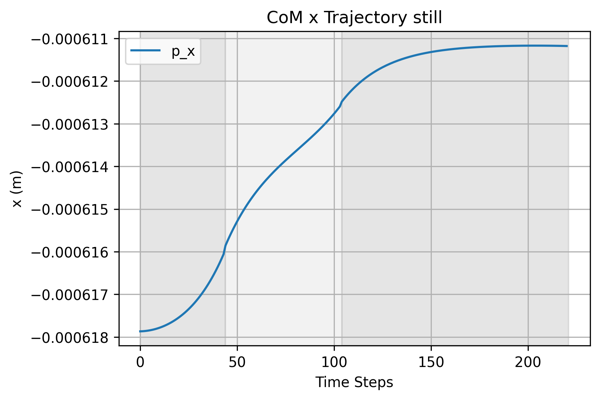
\includegraphics[width=\textwidth]{C:/Users/giuse/OneDrive/Desktop/GITHUB PROJECTS/AMR-FP1/centroidal_dyn-main/plots/CoM x Trajectory still.png}
        \caption{CoM x component}
        \label{fig:com_x_still}
    \end{subfigure}
    \hfill
    \begin{subfigure}[b]{0.32\textwidth}
        \centering
        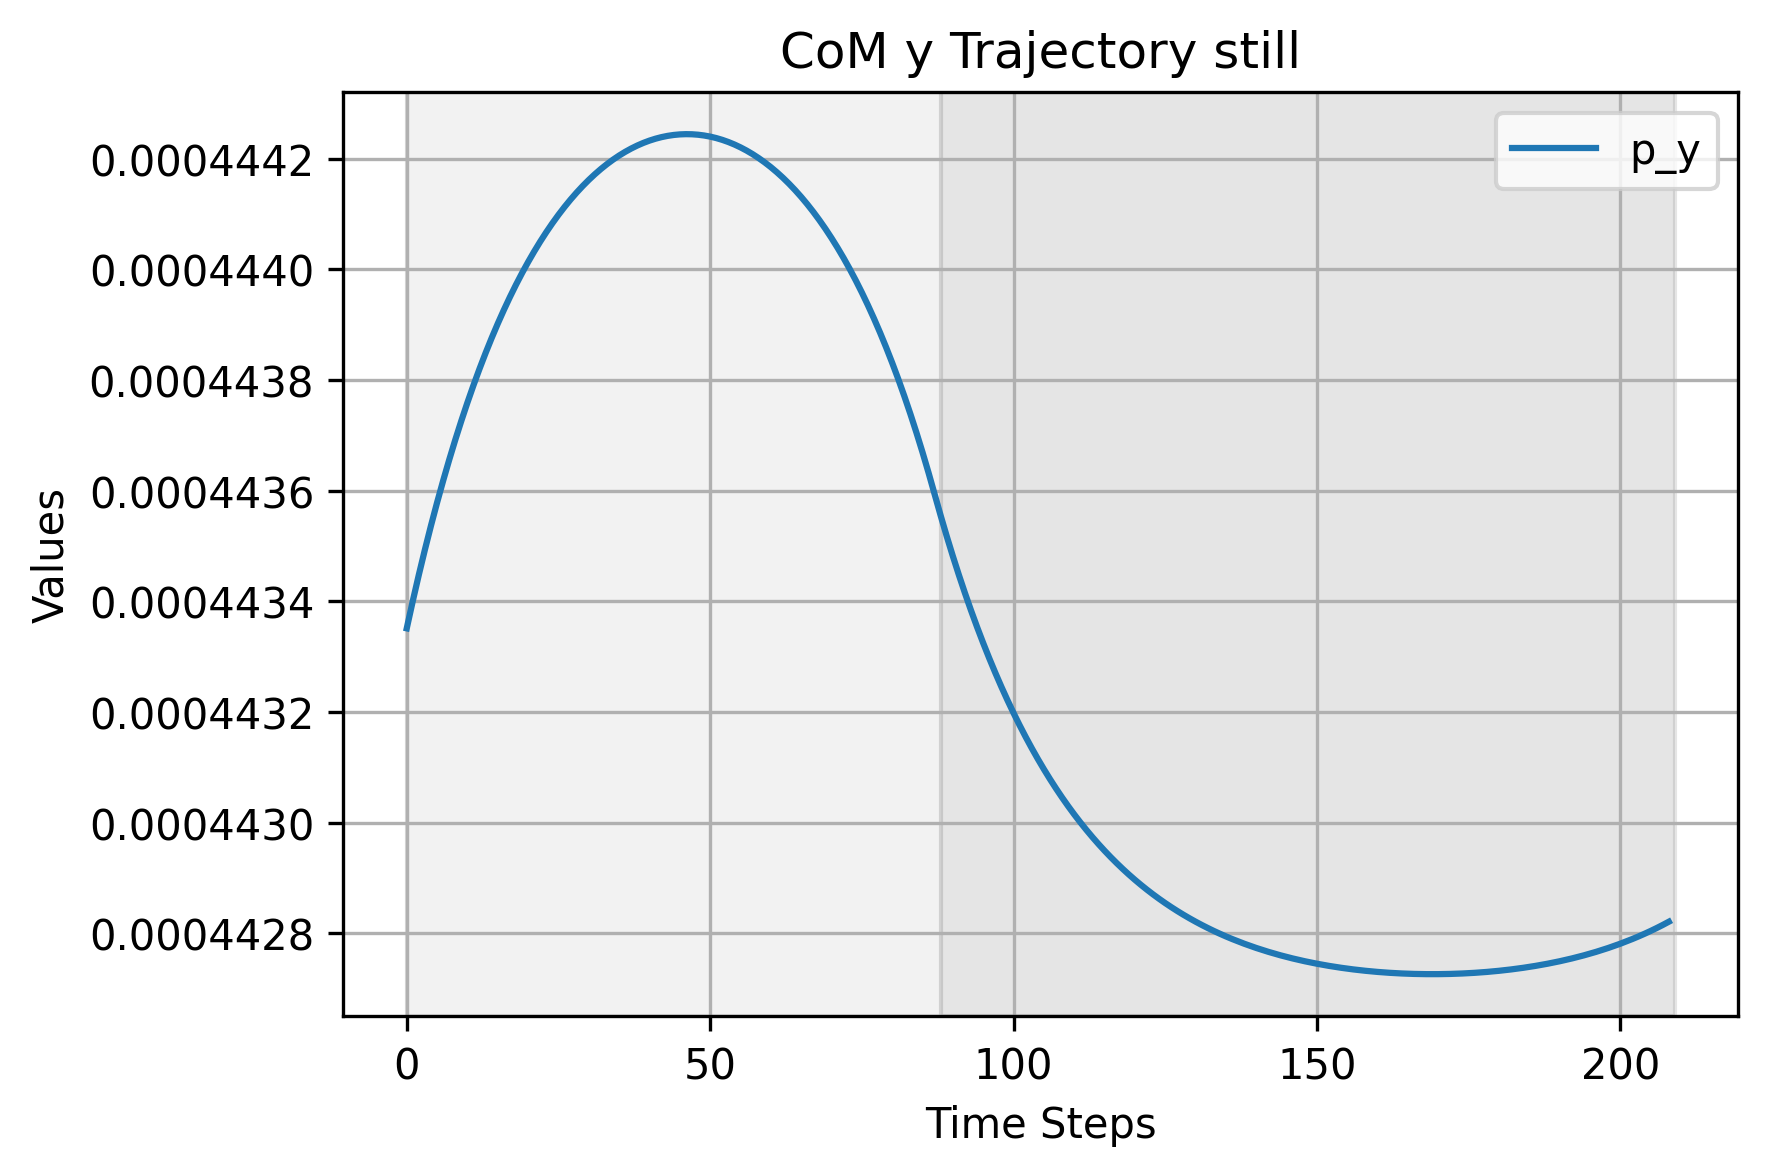
\includegraphics[width=\textwidth]{C:/Users/giuse/OneDrive/Desktop/GITHUB PROJECTS/AMR-FP1/centroidal_dyn-main/plots/CoM y Trajectory still.png}
        \caption{CoM y component}
        \label{fig:com_y_still}
    \end{subfigure}
    \hfill
    \begin{subfigure}[b]{0.32\textwidth}
        \centering
        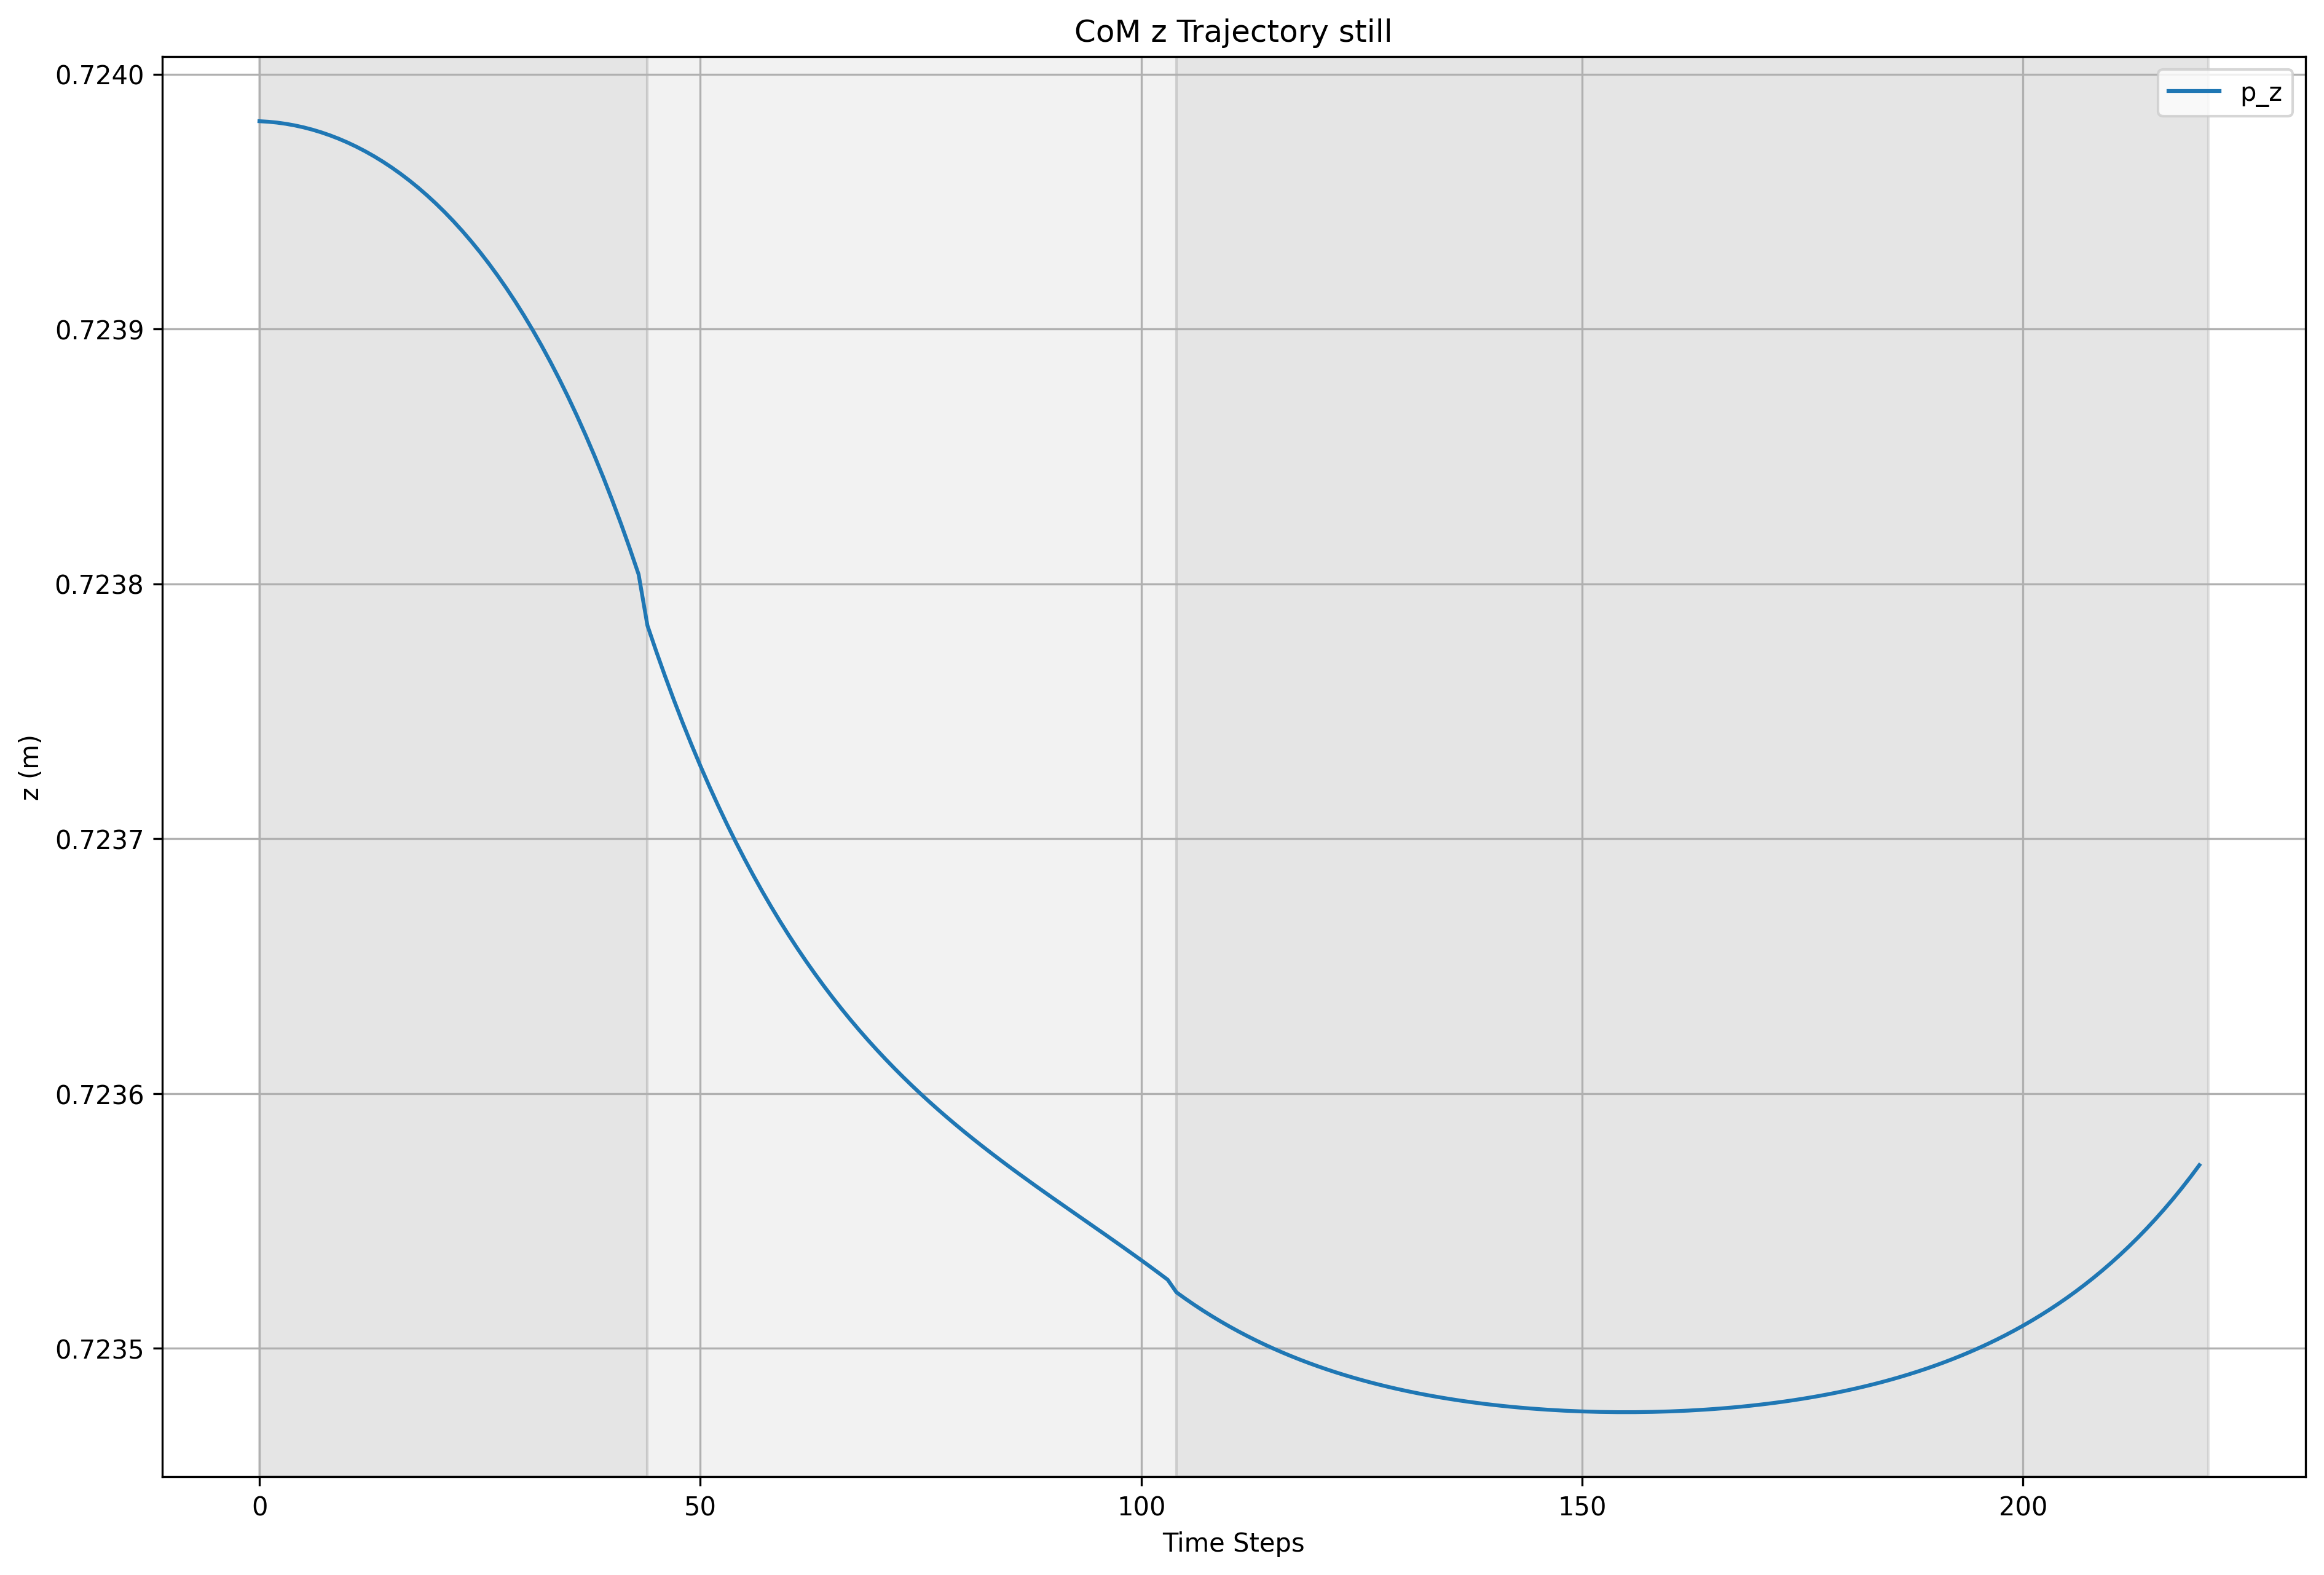
\includegraphics[width=\textwidth]{C:/Users/giuse/OneDrive/Desktop/GITHUB PROJECTS/AMR-FP1/centroidal_dyn-main/plots/CoM z Trajectory still.png}
        \caption{CoM z component}
        \label{fig:com_z_still}
    \end{subfigure}
    \caption{Evolution of CoM Position - Still Task}
    \label{fig:com_still}
\end{figure}
Fig.\ref{fig:three_still} shows the evolution of foot positions along the zz-axis, CoM velocity, and angular momentum during the still task. The foot positions in Fig. \ref{fig:feet_z_still} remain nearly constant, indicating minimal vertical motion. In Fig. \ref{fig:com_velocity_still}, slight oscillations in the $y$ and $z$ velocity components suggest minor corrective actions to maintain stability. The angular momentum in Fig. \ref{fig:angular_momentum_still} displays brief periodic drops, before returning to zero. This behavior indicates small adjustments to counteract any residual moments, ultimately preserving the robot’s stationary configuration. \\
\begin{figure}[htbp]
    \centering
    \begin{subfigure}[b]{0.32\textwidth}
        \centering
        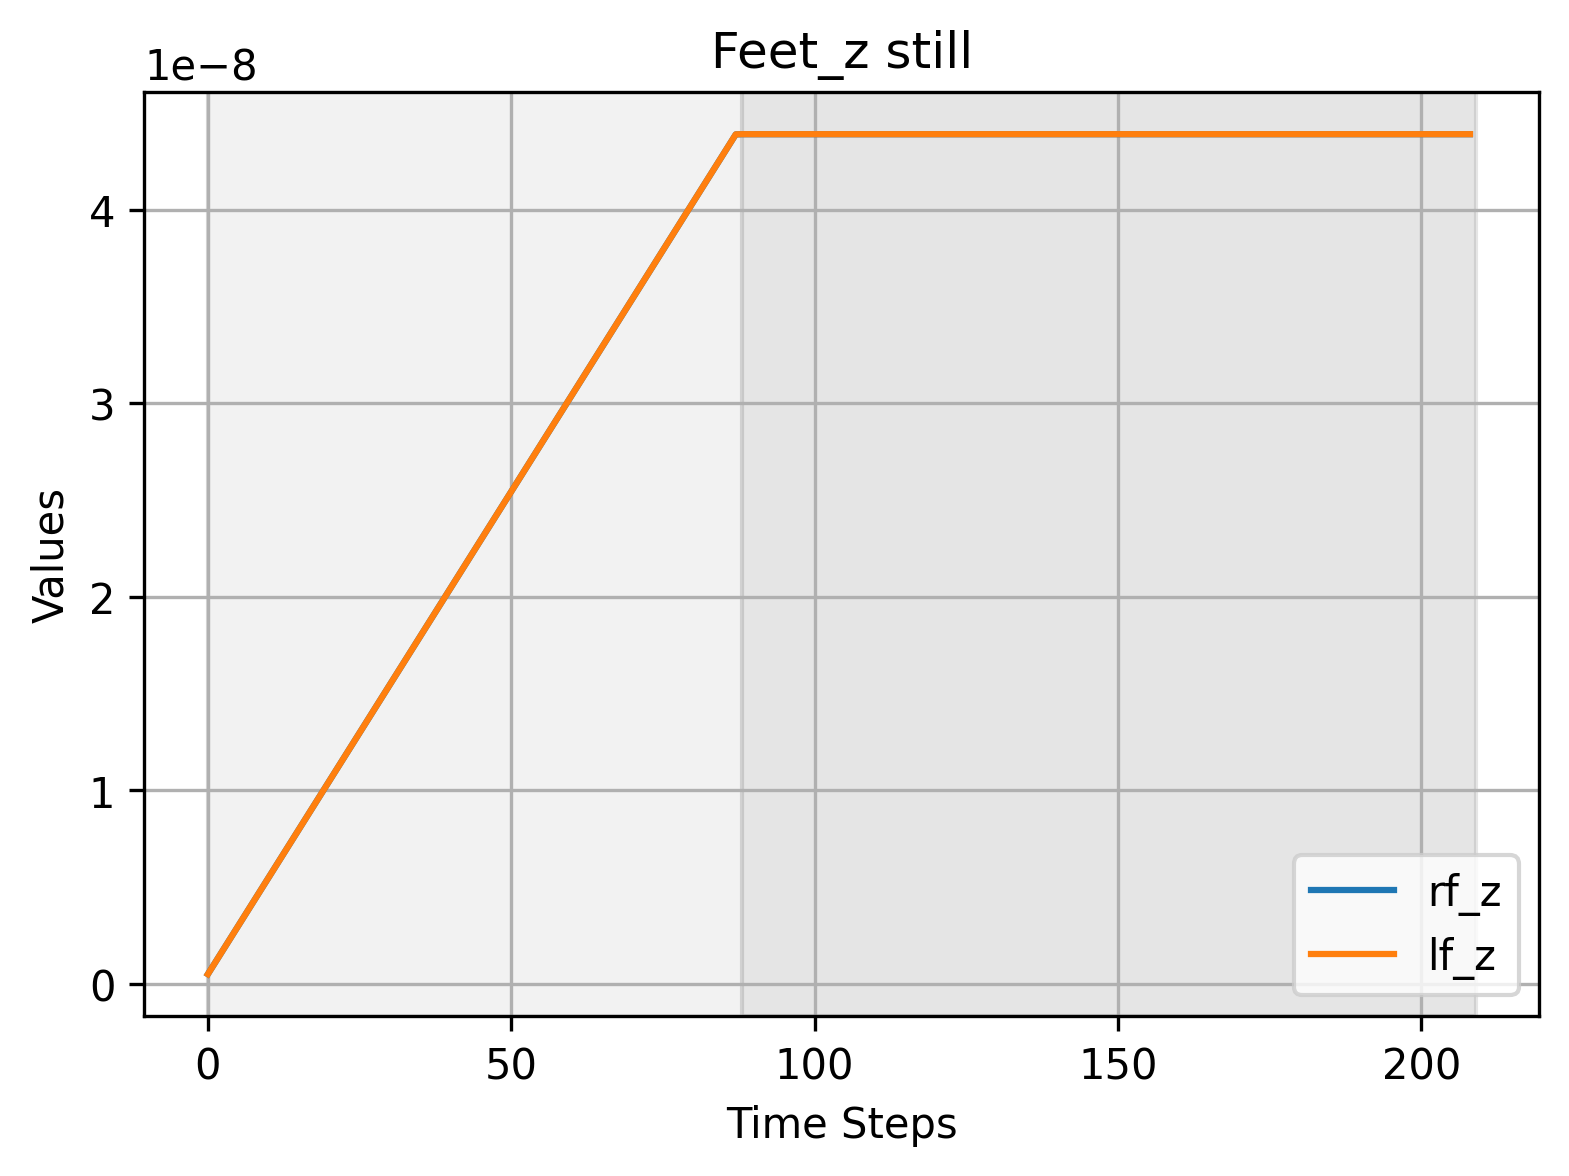
\includegraphics[width=\textwidth]{C:/Users/giuse/OneDrive/Desktop/GITHUB PROJECTS/AMR-FP1/centroidal_dyn-main/plots/Feet_z still.png}
        \caption{Feet along z axis}
        \label{fig:feet_z_still}
    \end{subfigure}
    \hfill
    \begin{subfigure}[b]{0.32\textwidth}
        \centering
        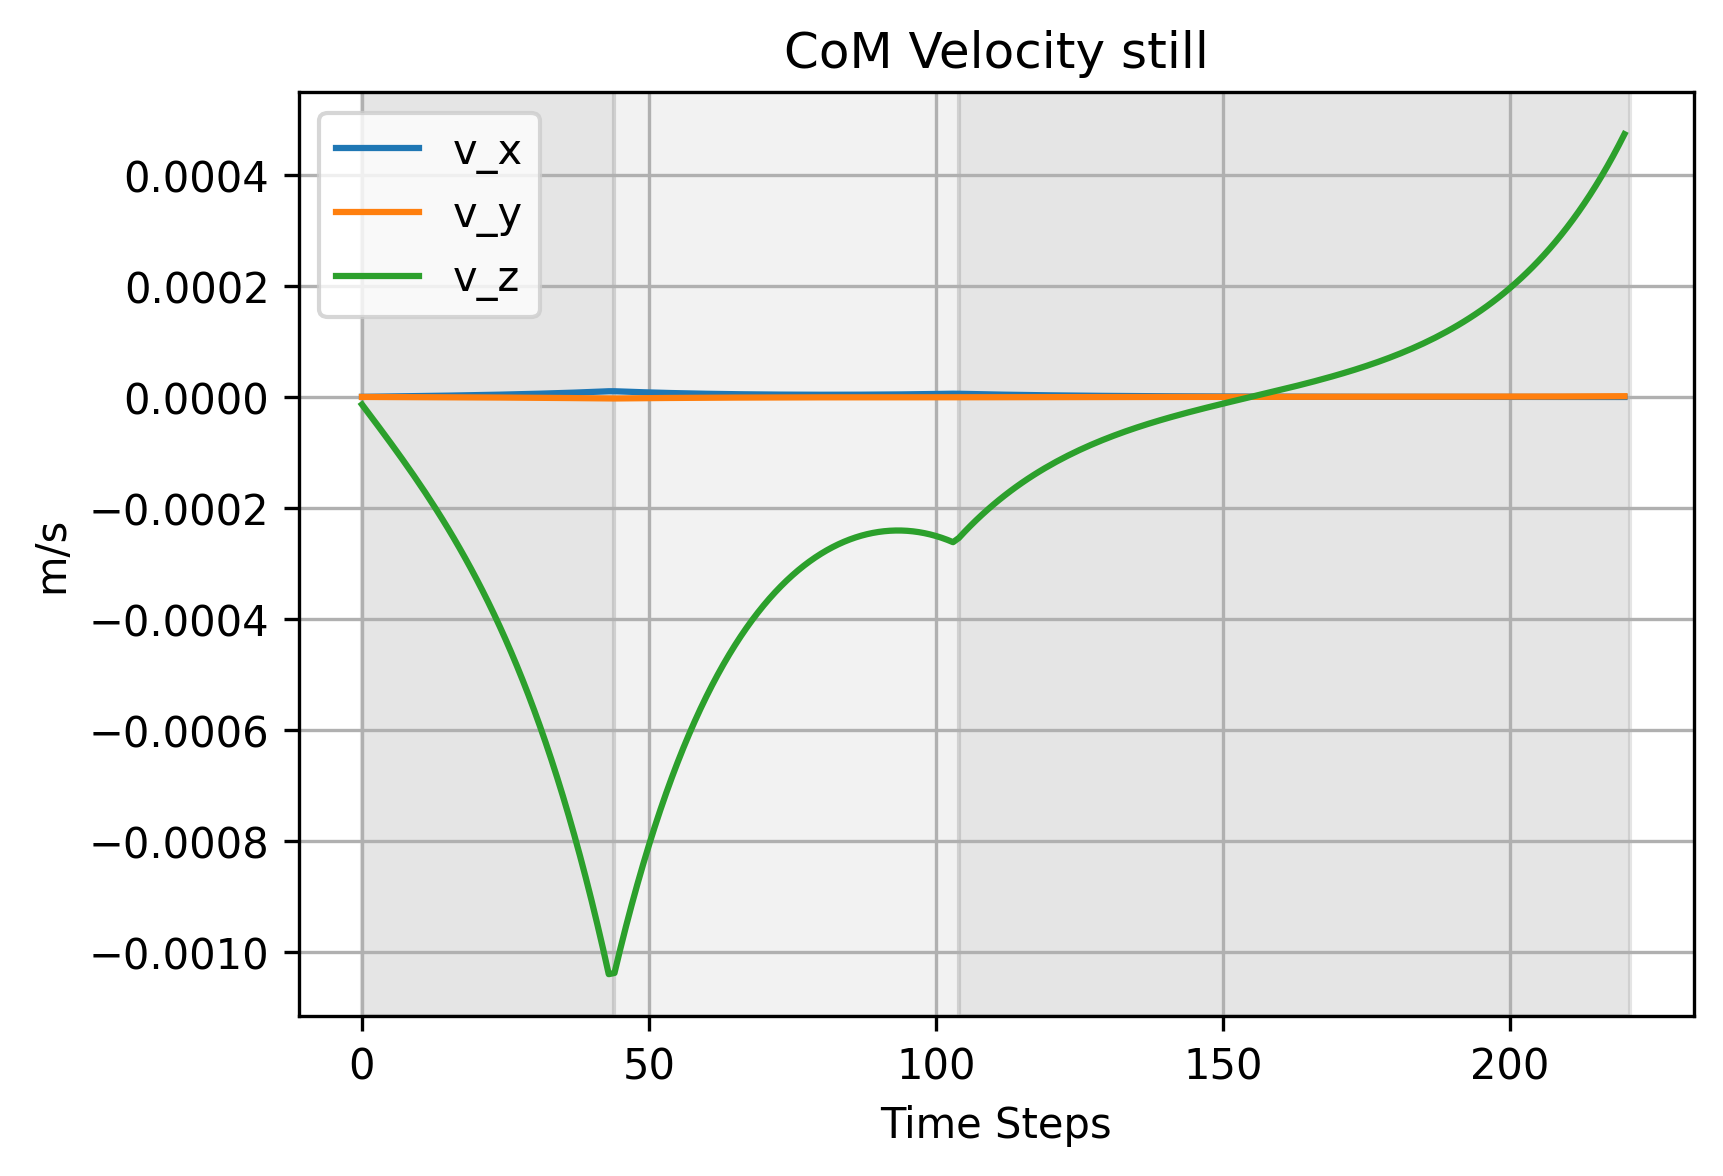
\includegraphics[width=\textwidth]{C:/Users/giuse/OneDrive/Desktop/GITHUB PROJECTS/AMR-FP1/centroidal_dyn-main/plots/CoM Velocity still.png}
        \caption{CoM Velocity}
        \label{fig:com_velocity_still}
    \end{subfigure}
    \hfill
    \begin{subfigure}[b]{0.32\textwidth}
        \centering
        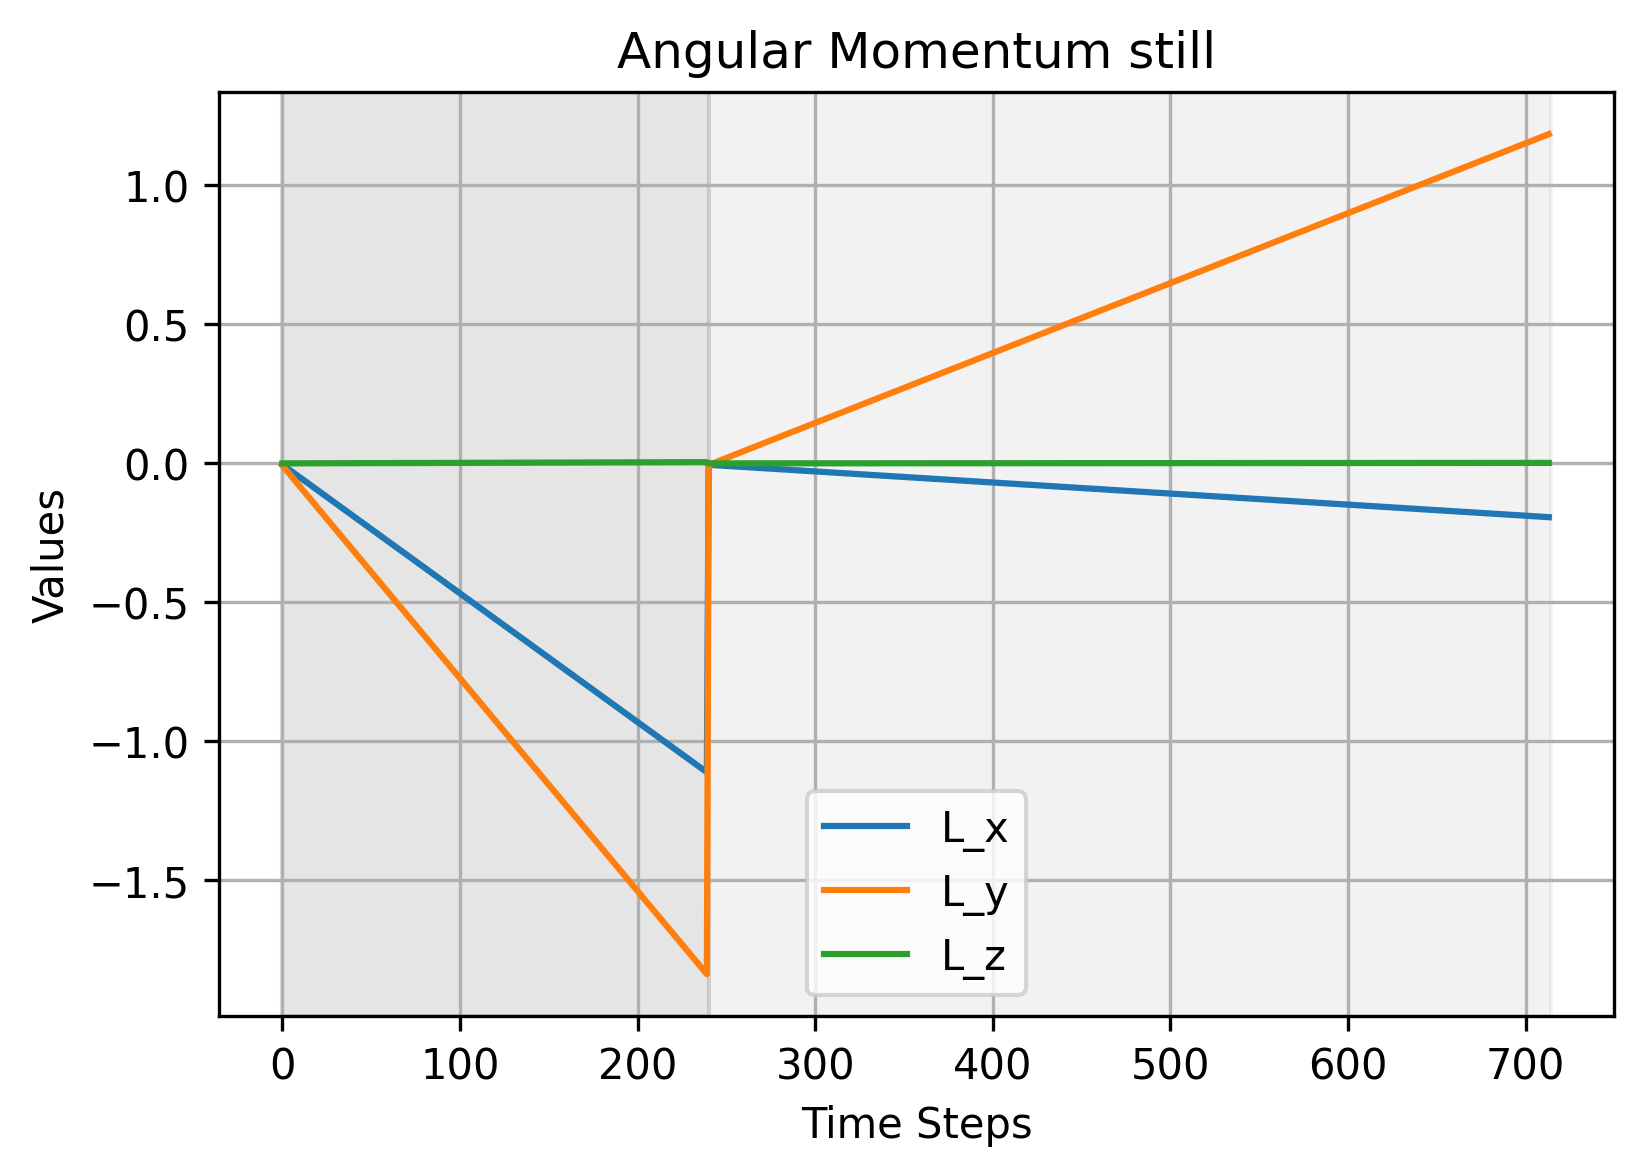
\includegraphics[width=\textwidth]{C:/Users/giuse/OneDrive/Desktop/GITHUB PROJECTS/AMR-FP1/centroidal_dyn-main/plots/Angular Momentum still.png}
        \caption{Angular Momentum}
        \label{fig:angular_momentum_still}
    \end{subfigure}
    \caption{Feet, Com Velocity and Angular Momentum - Still Task}
    \label{fig:three_still}
\end{figure}
\\
In Fig. \ref{fig:comparison_still} , the comparison between the reference and optimized trajectories for the still task is presented. The CoM position remains largely aligned with the reference values, with slight deviations observed primarily in the $x$ and $z$ components, reflecting minor adjustments to maintain stability. CoM velocity remains close to zero, consistent with the stationary objective, though minor oscillations indicate corrective actions against gravitational forces. Angular momentum shows small linear trends, particularly in the $x$ and $y$ components, suggesting residual moments being counteracted. Foot positions and velocities remain effectively constant, confirming that the feet maintain their initial stance without significant movement. Overall, the optimized trajectories exhibit minimal divergence from the reference, indicating effective stabilization while accounting for minor corrections.
\begin{figure}[htbp]
    \centering
    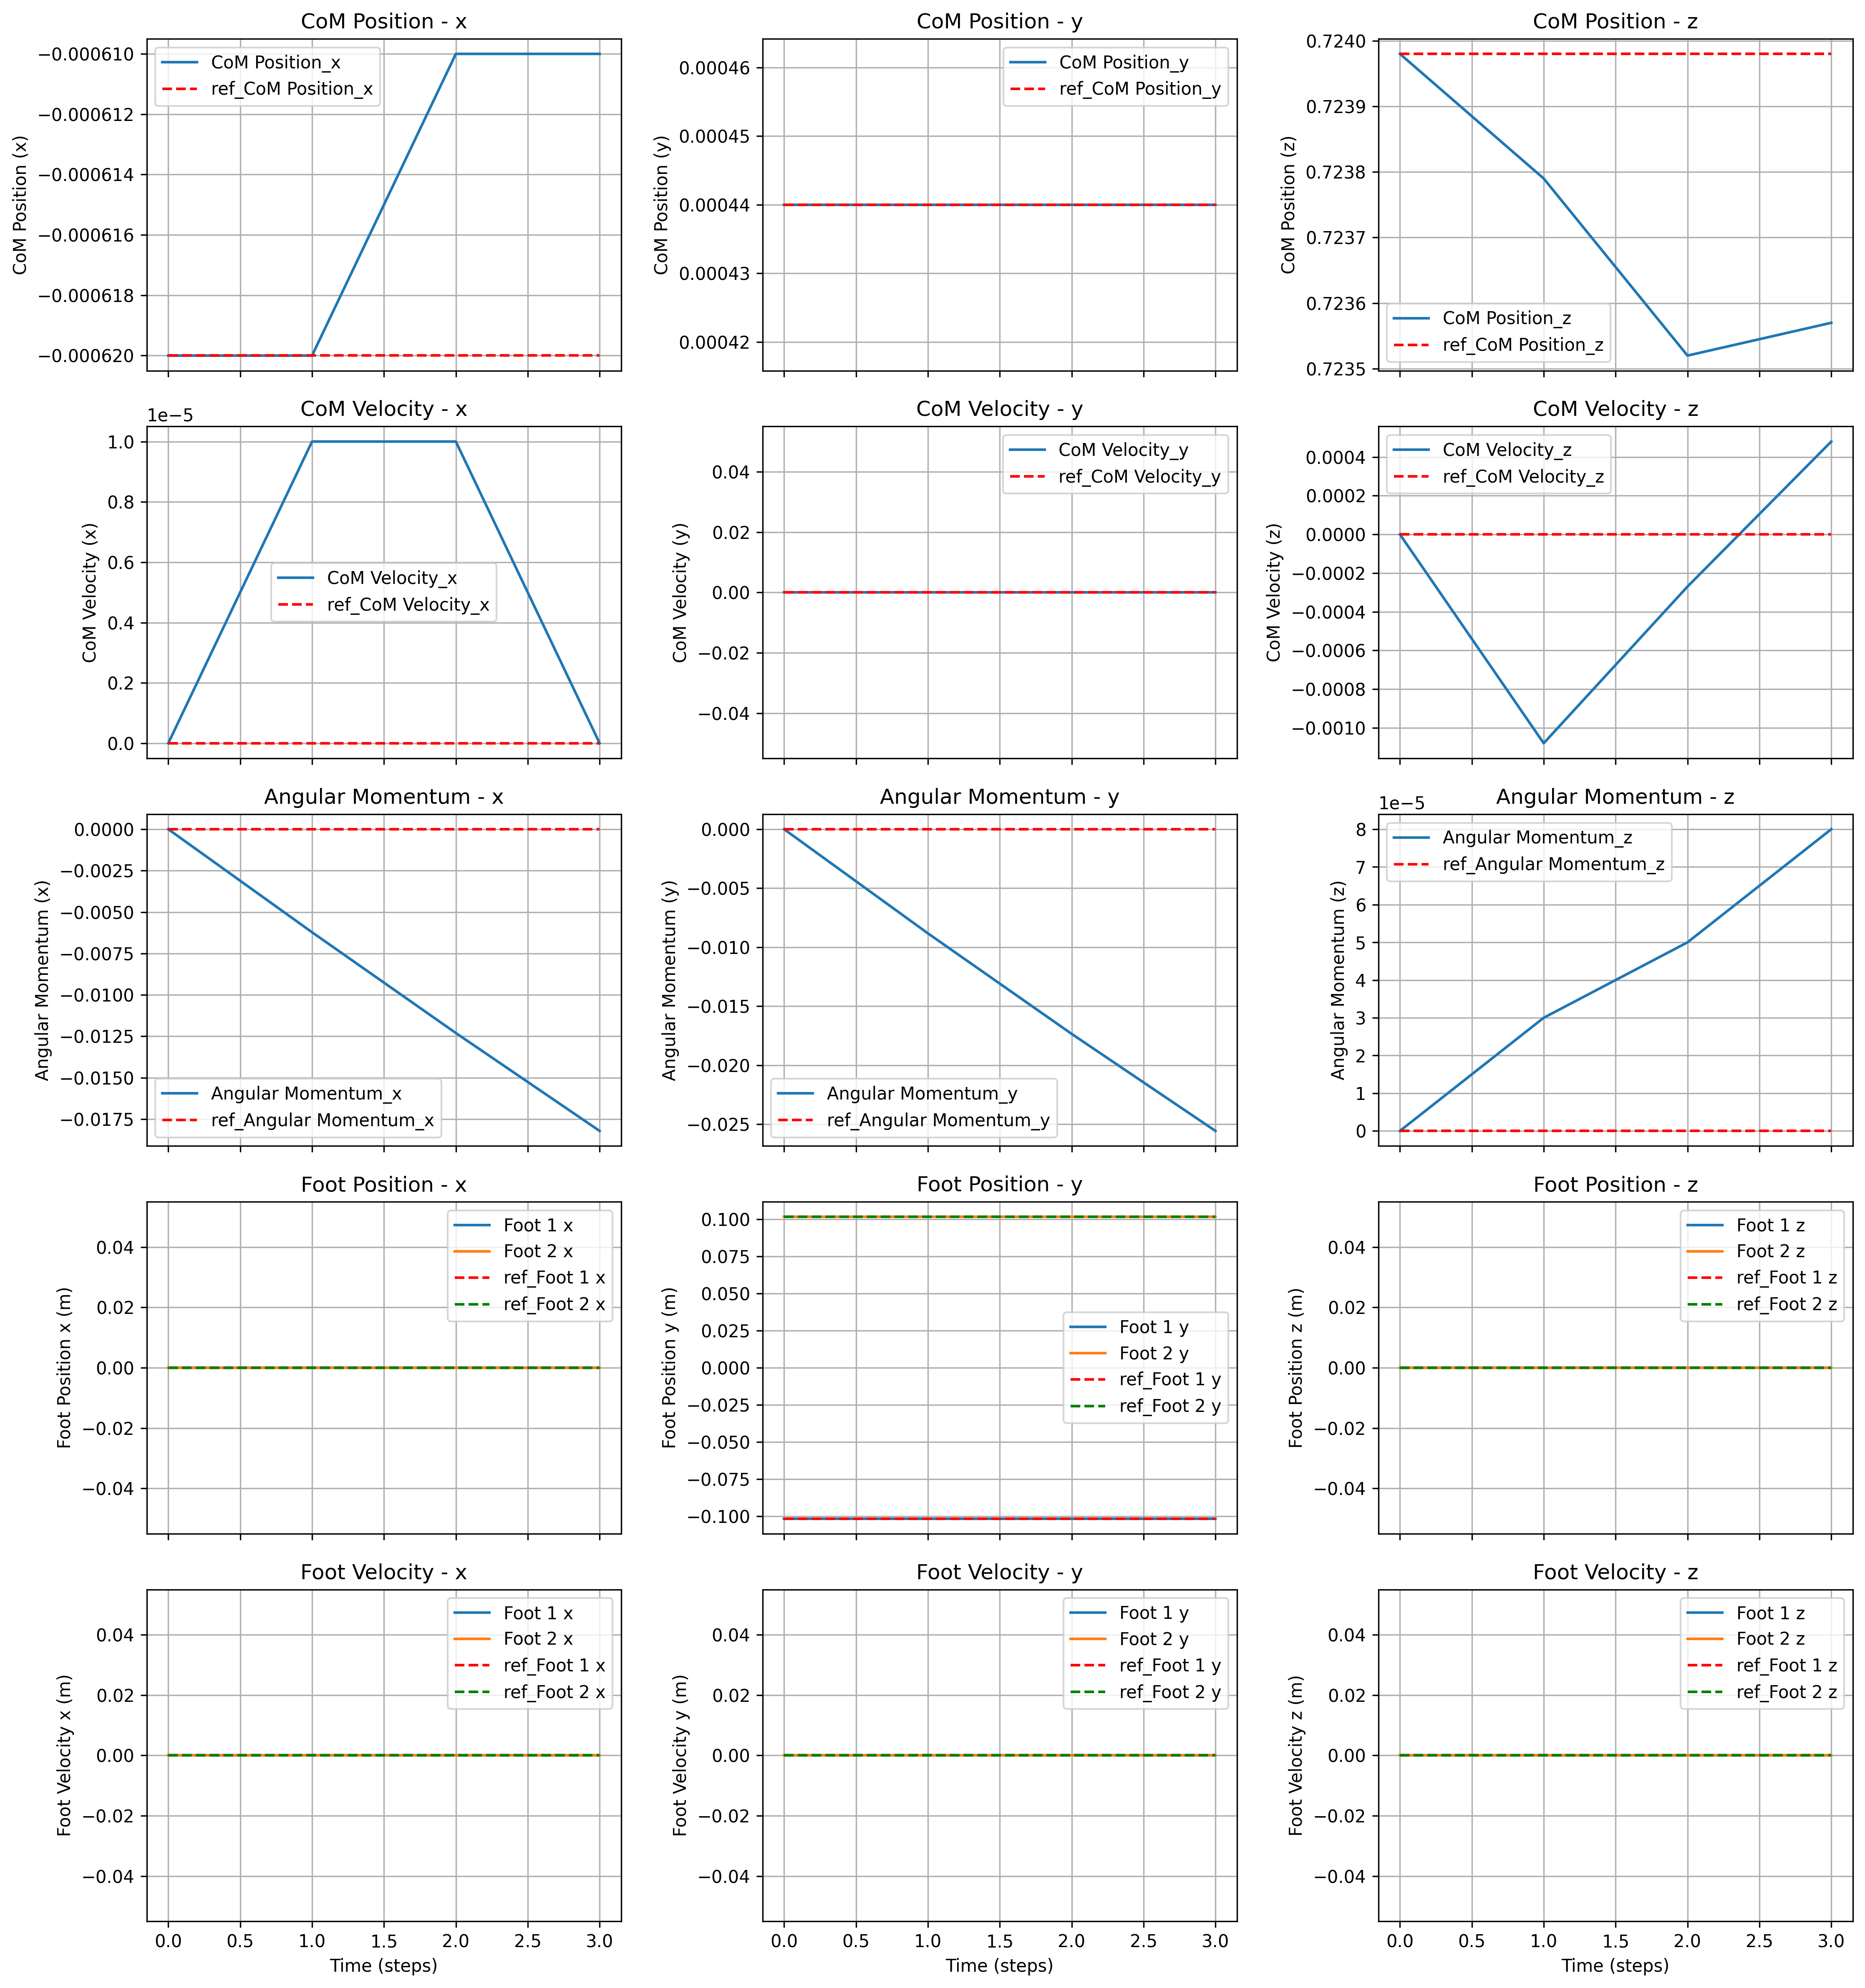
\includegraphics[width=0.8\textwidth]{C:/Users/giuse/OneDrive/Desktop/GITHUB PROJECTS/AMR-FP1/centroidal_dyn-main/plots/contact_x_still.png}
    \caption{Trajectory vs Reference - Still Task}
    \label{fig:comparison_still}
\end{figure}
\\
Another key aspect of the dynamics involves the contact wrenches, which represent the mechanical forces and moments applied by contact points, such as the feet, on the robot or vice versa. To maintain dynamic balance, the reaction force along the $z$-axis must counteract the gravitational force acting on the robot’s mass. The contact forces from the environment on both feet are summarized in Table \ref{tab:forces_still}. As indicated, when both feet remain grounded, the gravitational force is evenly distributed between the left and right foot, ensuring stability.
\begin{table}[H]
    \centering
    \renewcommand{\arraystretch}{1.2}
    \resizebox{\textwidth}{!}{
        \begin{tabular}{c|c|c|c|c}
            \hline
            Interval & Right Foot (x,y,z) & Left Foot (x,y,z) & $\Sigma L_k$ & Sum Forces (x,y,z) \\
            \hline
            0 & (-0.0598, 10.005, 70.689) & (-0.0598, -9.920, 70.689) & (0, 0) & (-0.1196, 0.0855, 141.379) \\
            1 & (0.0002, 9.537, 48.988) & (0.0002, -9.537, 48.993) & (0, 0) & (0.0003, -0.0002, 97.980) \\
            2 & (-0.0002, 9.539, 49.085) & (-0.0001, -9.538, 49.090) & (0, 0) & (-0.0003, 0.0002, 98.174) \\
            \hline
        \end{tabular}
    }
    \caption{Summary of Forces and Foot Positions per Interval - Still Task}
    \label{tab:forces_still}
\end{table}
To conclude our analysis of the still task, Figures \ref{fig:contact_forces_still_right} and \ref{fig:contact_forces_still_left} illustrate how the translational and rotational forces behave at the contact points. Along the horizontal axes, translational forces remain near zero, confirming minimal lateral interaction with the ground. The vertical component primarily compensates for gravitational effects, with slight variations indicating minor adjustments to maintain equilibrium. Rotational forces exhibit subtle trends, particularly in the \( x \) and \( y \) components, suggesting ongoing corrections to counteract residual torques. The \( z \) component shows a gradual decline, aligning with the angular momentum behavior observed in previous plots.
\begin{figure}[htbp]
    \centering
    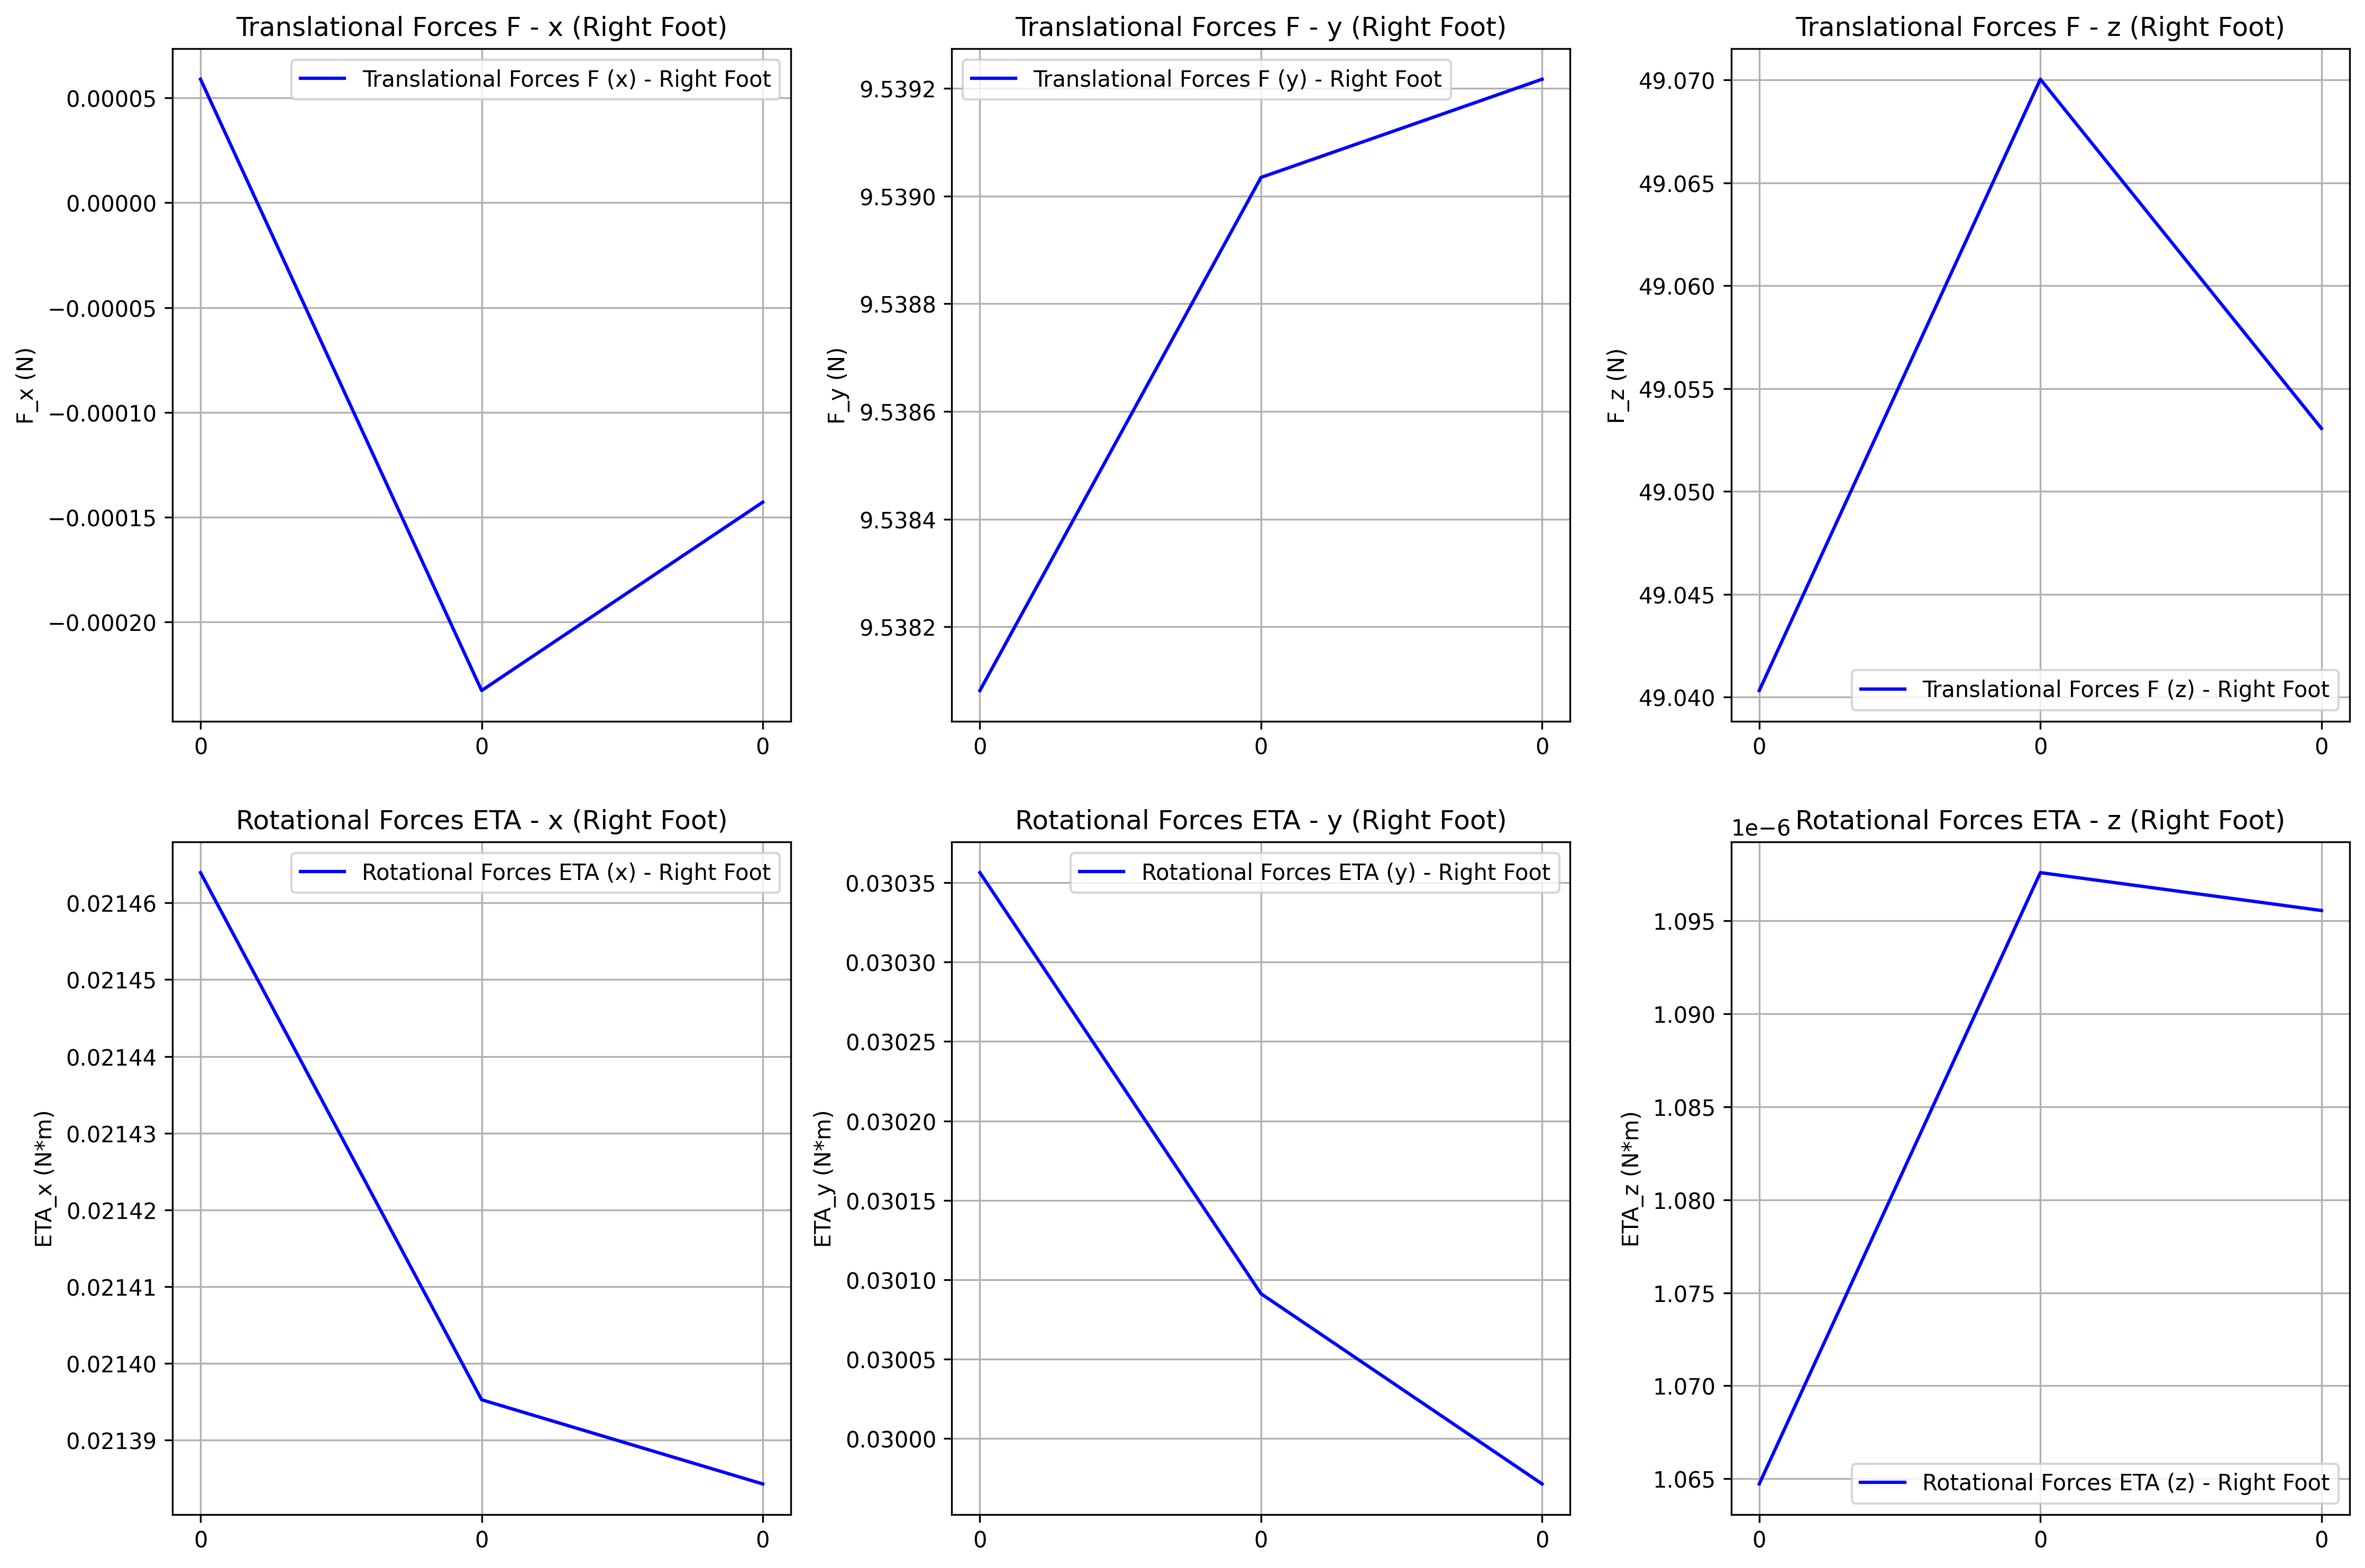
\includegraphics[width=0.8\textwidth]{C:/Users/giuse/OneDrive/Desktop/GITHUB PROJECTS/AMR-FP1/centroidal_dyn-main/plots/contact_forces_still_right.png}
    \caption{Trajectory vs Reference Forces Right Foot - Still Task}
    \label{fig:contact_forces_still_right}
\end{figure}
\begin{figure}[htbp]
    \centering
    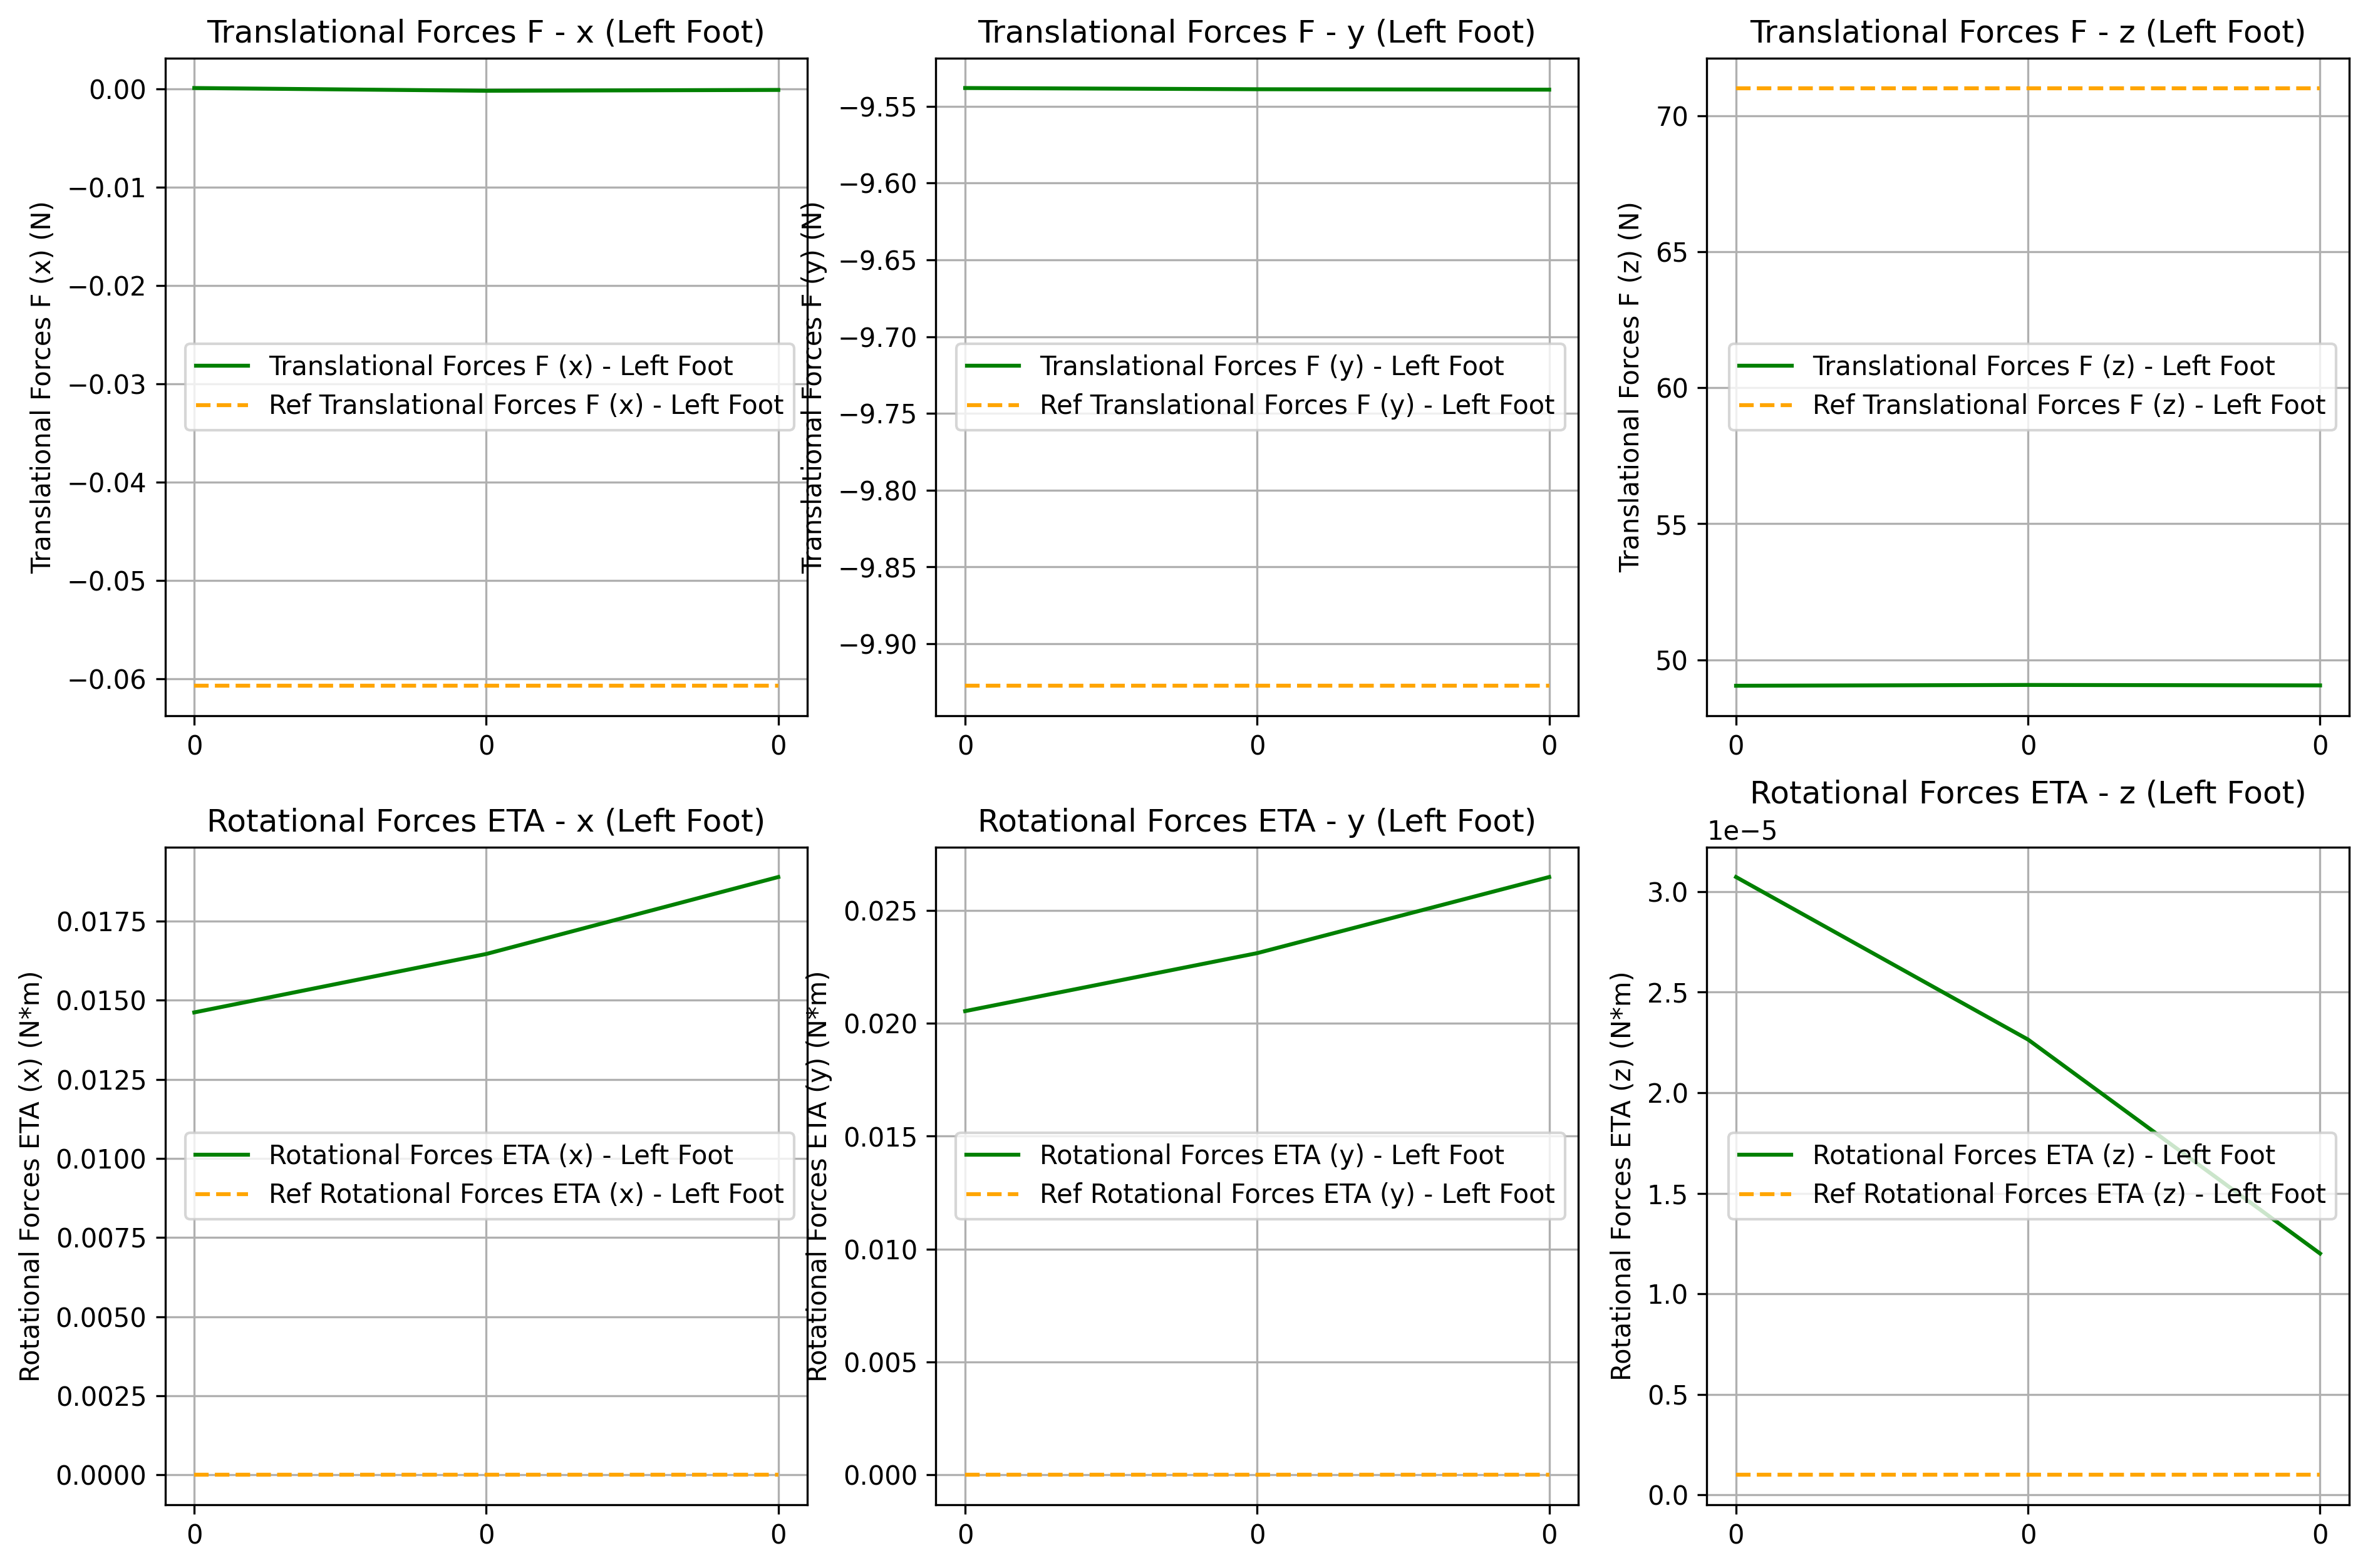
\includegraphics[width=0.8\textwidth]{C:/Users/giuse/OneDrive/Desktop/GITHUB PROJECTS/AMR-FP1/centroidal_dyn-main/plots/contact_forces_still_left.png}
    \caption{Trajectory vs Reference Forces Left Foot - Still Task}
    \label{fig:contact_forces_still_left}
\end{figure}
\newpage
\subsection{Walking Task}
Generalities about the walking task.

In the walking task, the trajectory is designed to simulate a natural walking pattern by coordinating the movements of the feet and the Center of Mass (CoM) through a sequence of double-support and single-support phases. During double-support phases, when both feet are in contact with the ground, the CoM remains stationary, providing stability. Movement along the X-axis occurs only during single-support phases, where one foot is lifted and the other remains grounded.

The CoM position update depends on the preceding phase. If the previous phase was double-support, the CoM remains at its current position. However, if the previous phase was single-support, the CoM advances by a specified displacement, ensuring consistent forward movement and balance.

The foot trajectory is constructed to simulate a natural step, where the foot in motion extends beyond the stationary foot. The Z-coordinate of each foot is set to zero at the start of each phase, representing ground contact. As the foot moves during the single-support phase, its height follows a parabolic profile, allowing for a smooth lift-off and descent. This profile is determined by interpolating between the start and end positions defined by the phase solutions, ensuring continuity and preventing abrupt changes.

Furthermore, the X-coordinate of the moving foot is updated alternately, depending on which foot was lifted in the previous phase. This alternating pattern maintains rhythmic progression, effectively mimicking a natural walking cycle. Consequently, the contact sequence, as presented in Table 2, defines the specific sequence of double-support and single-support phases, guiding the transitions and timing of each step.

\begin{table}[h!]
    \label{tab:walkingtask}
    \centering
    \begin{tabular}{|c|c|c|c|}
        \hline
        Task & N & Foot & Contact Sequence \\
        \hline
        Walk & 24 & Right & 000-000-000-000-000-0 \\
        & & Left & 0-000-000-000-000-000 \\
        \hline
    \end{tabular}
    \caption{Contact sequence - Walking task}
\end{table}



\paragraph{Reference Trajectory Generation}
\begin{algorithm}[H]
\caption{Reference Trajectory Generation - Walking Task}
\label{alg:walking_task}
\textbf{Input:} Number of effectors ($n_e$), Number of timesteps ($N$), Contact sequence ($\sigma$) \\
\textbf{Output:} Reference state matrix ($X_{ref}$), Reference control matrix ($U_{ref}$)

\begin{algorithmic}[1]
\State \textbf{Initialize:}
\State Set $time_k \gets 0$
\State Initialize $X_{ref}$ and $U_{ref}$ as zero matrices of appropriate sizes
\State Define initial CoM position, orientation, and velocity
\State Define initial foot positions and orientations

\State \textbf{Configure Contact Phases:}
\For{$t = 1$ to $N$}
    \State Extract right and left contact states from $\sigma$
    \State Determine phase duration and contact forces:
    \If{right foot in swing ($right = -1$, $left = 0$)}
        \State $phase\_duration \gets 1$
        \State $\lambda_{right} \gets 0$
        \State $\lambda_{left} \gets \sqrt{\frac{9.81}{0.5}}$
    \ElsIf{left foot in swing ($left = -1$, $right = 0$)}
        \State $phase\_duration \gets 1$
        \State $\lambda_{left} \gets 0$
        \State $\lambda_{right} \gets \sqrt{\frac{9.81}{0.5}}$
    \Else
        \State $phase\_duration \gets 1$
        \State $\lambda_{right}, \lambda_{left} \gets \sqrt{9.81}$
    \EndIf
    \State Store $phase\_duration$ and contact forces in $U_{ref}$
\EndFor

\State \textbf{Update States:}
\For{$t = 1$ to $N$}
    \State Extract current contact states
    \State Determine velocities and displacements based on transitions (see Table \ref{tab:logic_walking})
    \State Update CoM position and velocity in $X_{ref}$
    \State Update foot positions based on calculated foot velocities
    \State Update $time_k$ based on $phase\_duration$
\EndFor

\State \textbf{Return:} $X_{ref}, U_{ref}$
\end{algorithmic}
\end{algorithm}

\begin{table}[H]
\centering
\renewcommand{\arraystretch}{1.2}
\caption{Detailed Logic for Setting Foot/CoM Velocities and Displacements}
\label{tab:logic_walking}
\begin{tabular}{|l|c|c|c|}
\hline
\textbf{Transition} & \textbf{CoM Velocity (x, y)} & \textbf{Foot Velocity (x, z)} & \textbf{Displacement (x, y, z)} \\
\hline
Right = -1, prev = 0 & (0, 0.07) & (0, 0) & (0, 0.07, 0) \\
Left = -1, prev = 0 & (0, -0.07) & (0, 0) & (0, -0.07, 0) \\
Right = 0, prev = -1 & (0.2, -0.07) & (0.1, 0) & (0.1, -0.07, 0) \\
Left = 0, prev = -1 & (0.2, 0.07) & (0.1, 0) & (0.1, 0.07, 0) \\
Default (both feet in contact) & (0.1, 0) & (0, 0) & (0.1, 0, 0) \\
\hline
\end{tabular}
\end{table}






\paragraph{Simulation Results}
Say something about the walking task and the results here. \\ 
In Figure 15, the evolution of the CoM position components (X, Y, Z) during the walking task is illustrated. The X component shows a consistent upward trend, representing the forward progression of the CoM as the robot advances step by step. This steady increase is expected, as the walking task involves continuous forward movement. \\
The Y component exhibits a pronounced oscillatory pattern, corresponding to the lateral sway that naturally occurs as the robot shifts its weight from one foot to the other during each step. The regularity of these oscillations reflects the cyclic nature of the walking gait, with each peak and trough aligning with foot contact transitions. \\
The Z component also follows a periodic oscillation, capturing the vertical motion as the feet alternate between ground contact and lift-off. The amplitude of these oscillations is relatively small, indicating that the CoM height remains fairly stable, with slight variations caused by the foot lift and placement during each step.
\begin{figure}[H]
    \centering
    \begin{subfigure}[b]{0.32\textwidth}
        \centering
        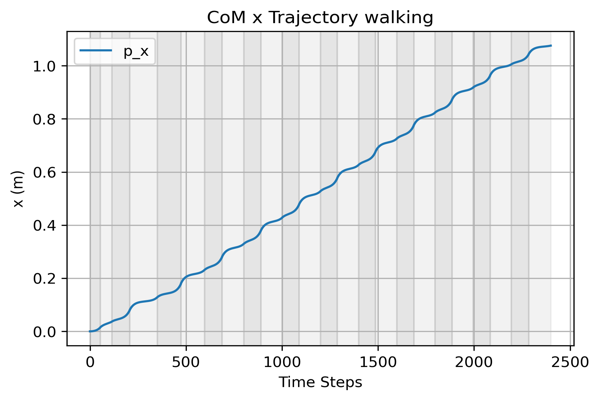
\includegraphics[width=\textwidth]{C:/Users/giuse/OneDrive/Desktop/GITHUB PROJECTS/AMR-FP1/centroidal_dyn-main/plots/CoM x Trajectory walking.png}
        \caption{CoM x component}
        \label{fig:sub1}
    \end{subfigure}
    \hfill
    \begin{subfigure}[b]{0.32\textwidth}
        \centering
        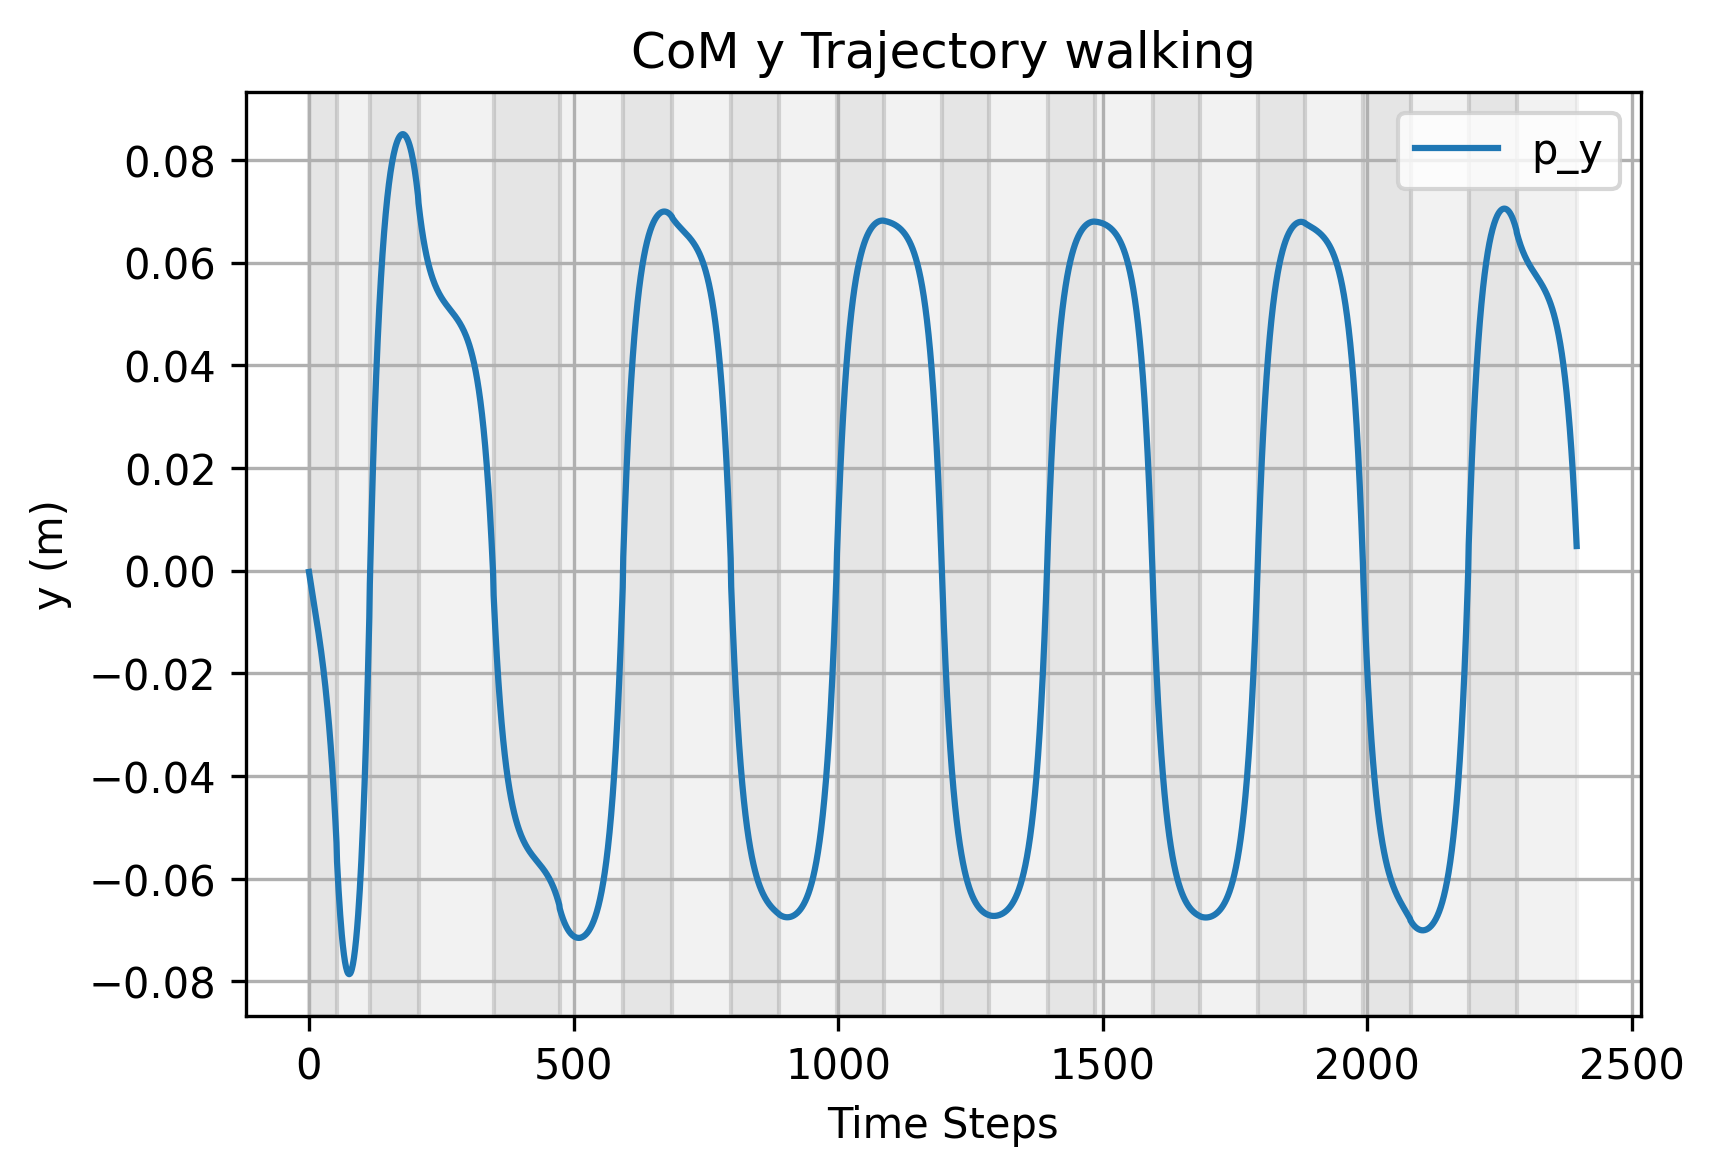
\includegraphics[width=\textwidth]{C:/Users/giuse/OneDrive/Desktop/GITHUB PROJECTS/AMR-FP1/centroidal_dyn-main/plots/CoM y Trajectory walking.png}
        \caption{CoM y component}
        \label{fig:sub2}
    \end{subfigure}
    \hfill
    \begin{subfigure}[b]{0.32\textwidth}
        \centering
        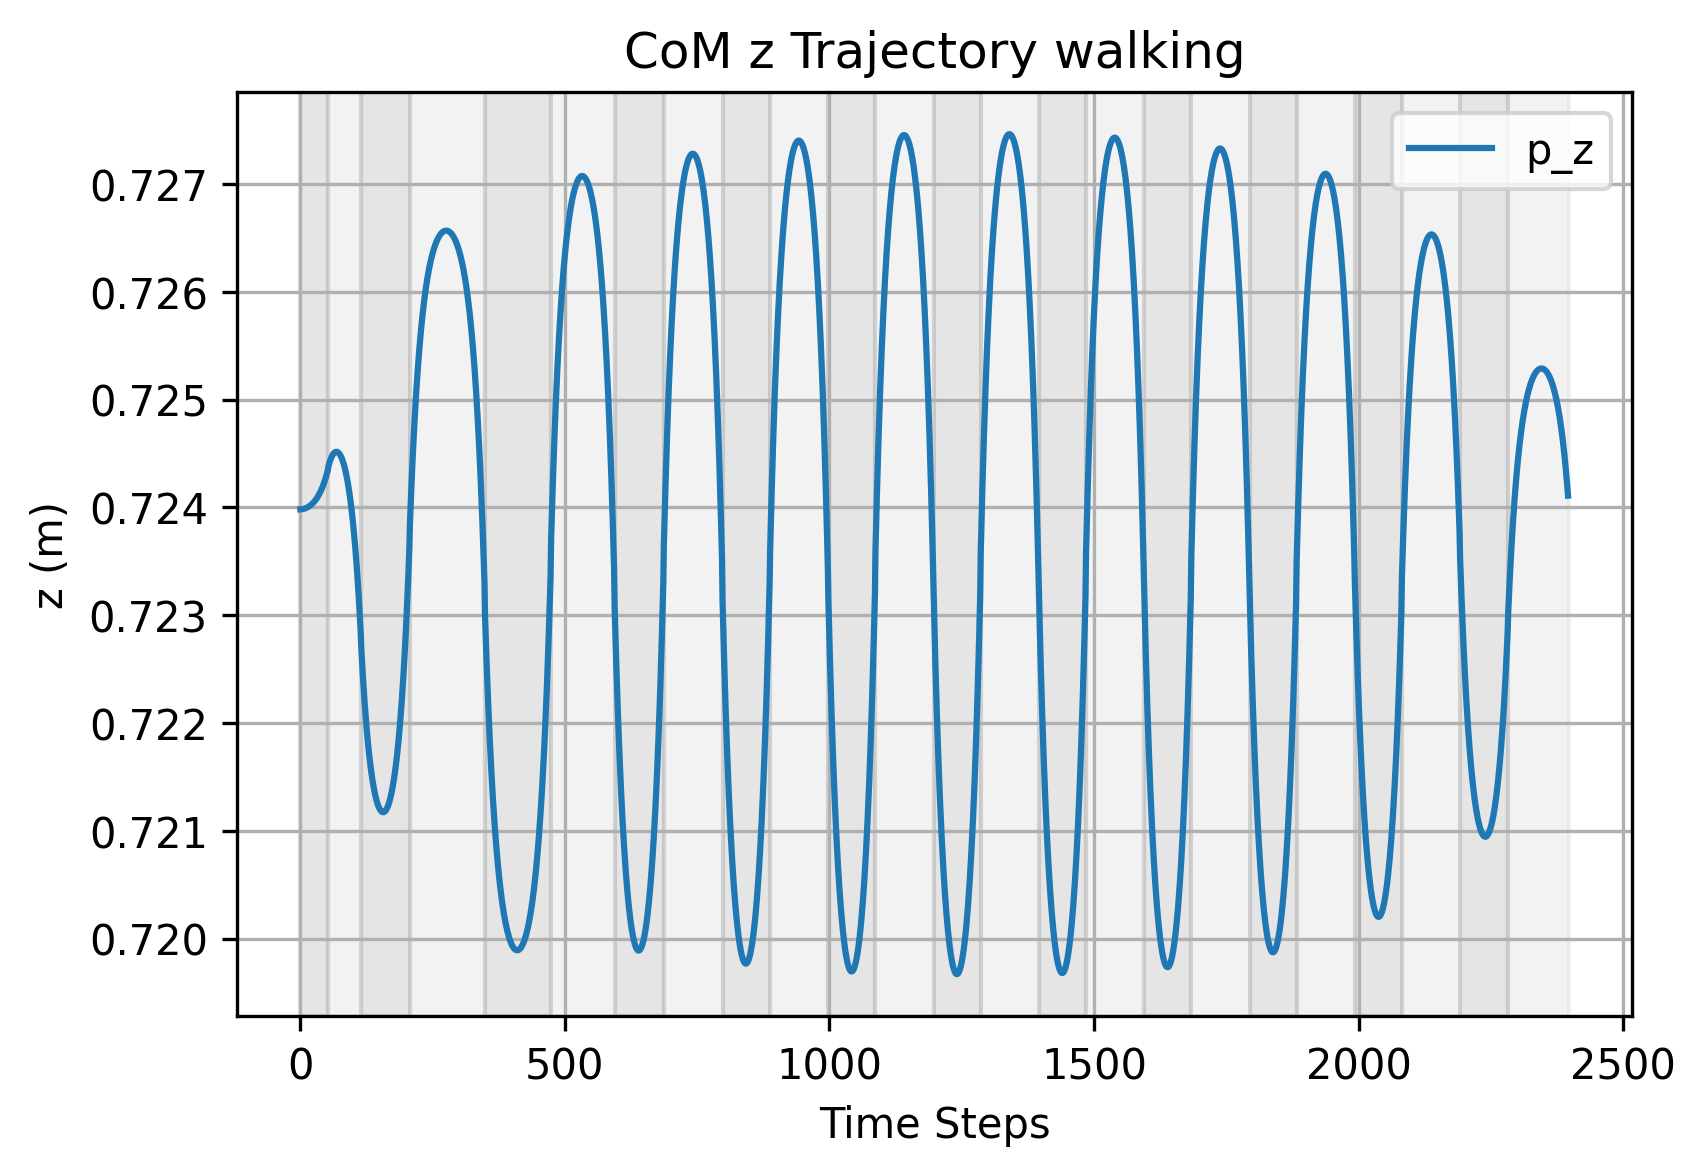
\includegraphics[width=\textwidth]{C:/Users/giuse/OneDrive/Desktop/GITHUB PROJECTS/AMR-FP1/centroidal_dyn-main/plots/CoM z Trajectory walking.png}
        \caption{CoM z component}
        \label{fig:sub3}
    \end{subfigure}
    \caption{Evolution of CoM Position - Walking Task}
    \label{fig:threeimages}
\end{figure}
In Figure 16, the evolution of the feet positions along the Z-axis, CoM velocity, and angular momentum during the walking task is presented.\\
The Z-axis foot positions exhibit periodic oscillations, representing the alternating lift-off and ground contact of each foot as the robot progresses through the walking gait. The regular pattern confirms the cyclic nature of the stepping sequence, with each peak corresponding to a foot being lifted and each trough indicating ground contact.\\
The CoM velocity components display distinct oscillatory patterns, with pronounced fluctuations in the X direction due to forward movement and periodic variations in the Y and Z components corresponding to lateral and vertical adjustments during each step. The consistent oscillations align with the alternating support phases and reflect the dynamic nature of walking.\\
The angular momentum components (Lx, Ly, Lz) show noticeable oscillations, particularly in the X component, indicating significant torques generated during each step to maintain balance and control. The cyclic nature of these oscillations is consistent with the alternating foot contact, highlighting the system’s continuous adjustments to maintain stability throughout the walking cycle.
\begin{figure}[htbp]
    \centering
    \begin{subfigure}[b]{0.32\textwidth}
        \centering
        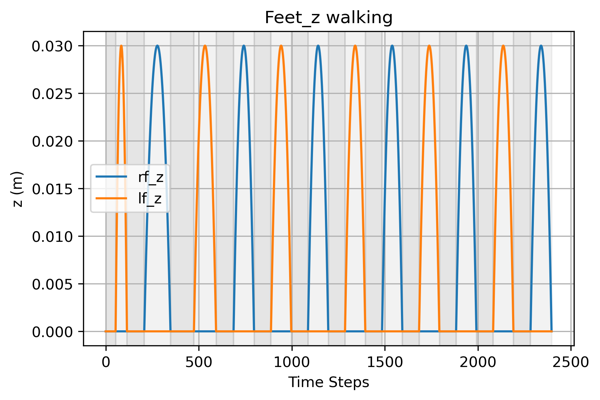
\includegraphics[width=\textwidth]{C:/Users/giuse/OneDrive/Desktop/GITHUB PROJECTS/AMR-FP1/centroidal_dyn-main/plots/Feet_z walking.png}
        \caption{Feet along z axis}
        \label{fig:sub1}
    \end{subfigure}
    \hfill
    \begin{subfigure}[b]{0.32\textwidth}
        \centering
        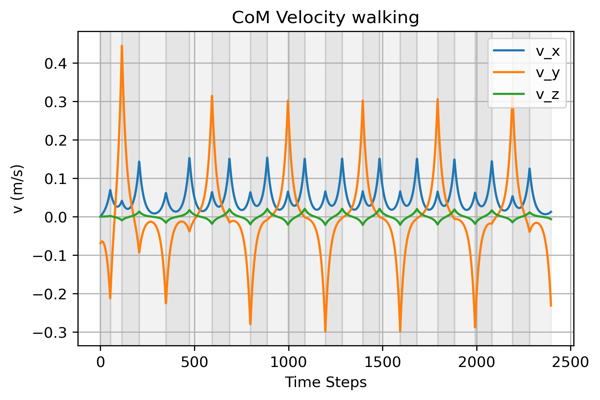
\includegraphics[width=\textwidth]{C:/Users/giuse/OneDrive/Desktop/GITHUB PROJECTS/AMR-FP1/centroidal_dyn-main/plots/CoM Velocity walking.png}
        \caption{CoM Velocity}
        \label{fig:sub2}
    \end{subfigure}
    \hfill
    \begin{subfigure}[b]{0.32\textwidth}
        \centering
        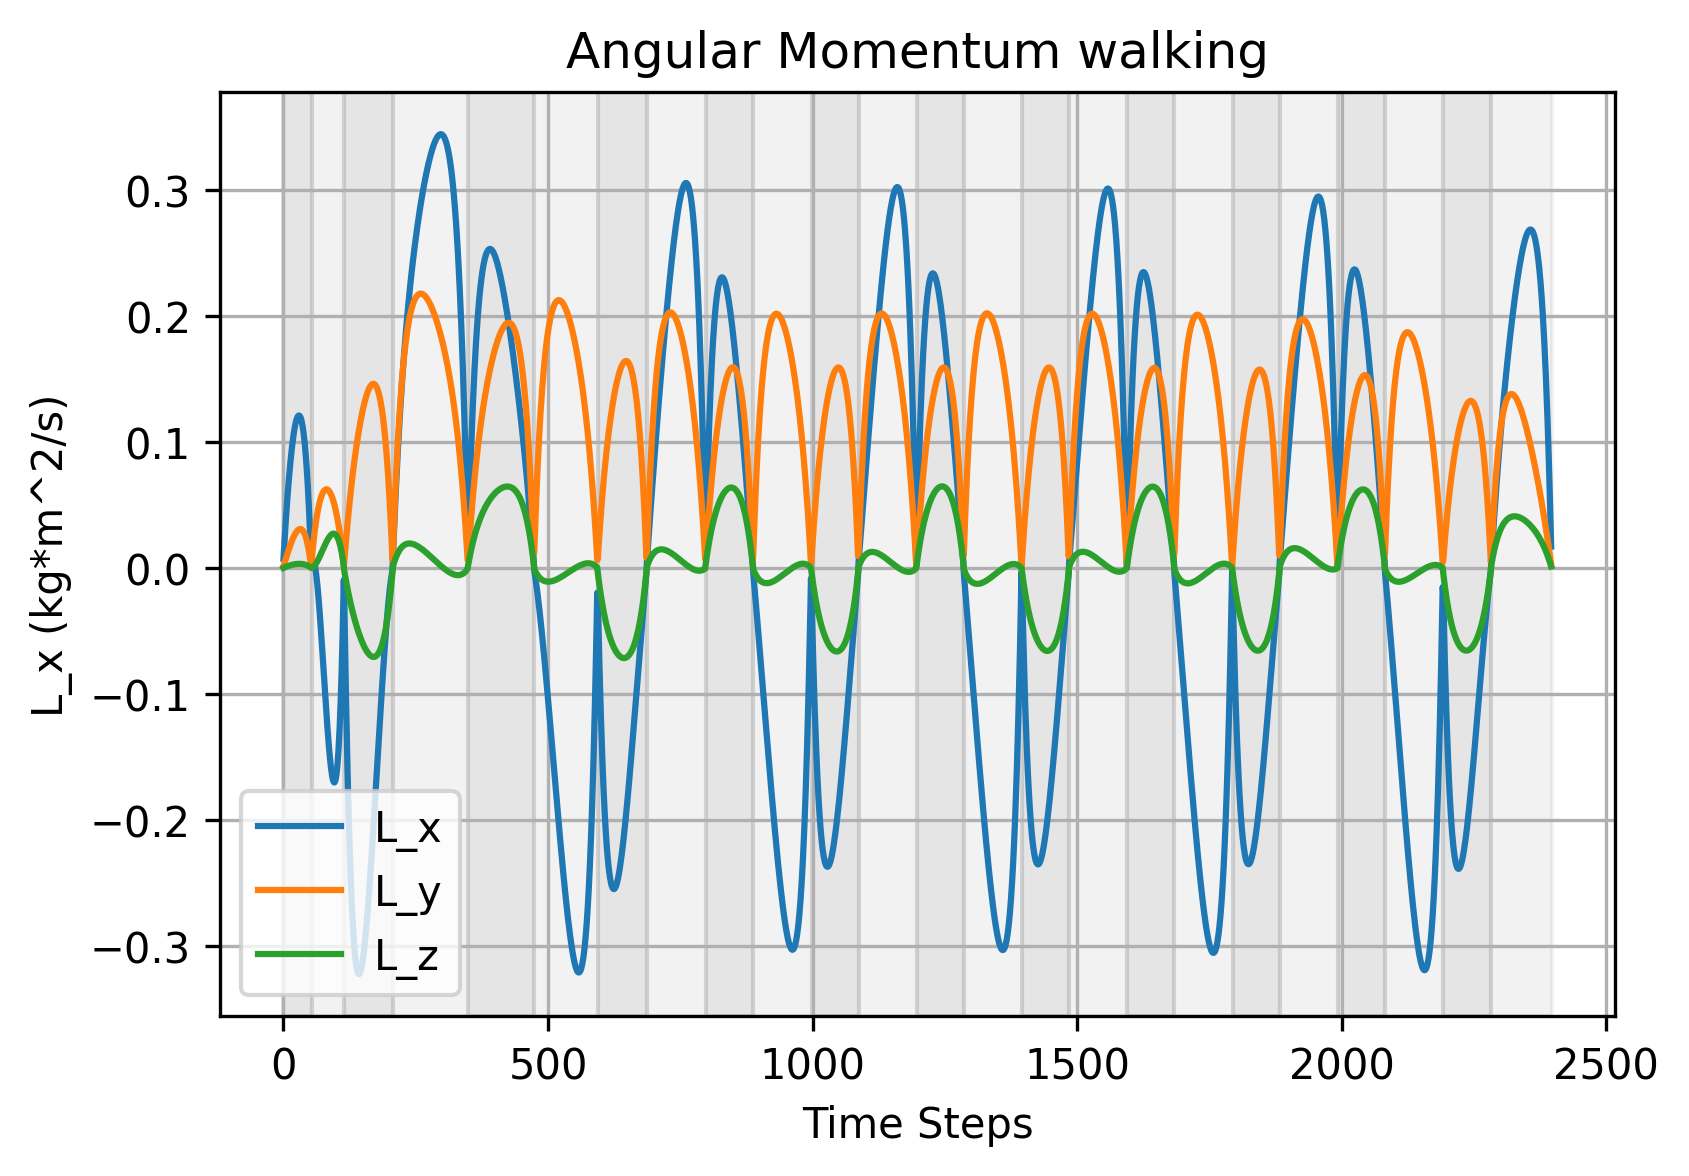
\includegraphics[width=\textwidth]{C:/Users/giuse/OneDrive/Desktop/GITHUB PROJECTS/AMR-FP1/centroidal_dyn-main/plots/Angular Momentum walking.png}
        \caption{Angular Momentum}
        \label{fig:sub3}
    \end{subfigure}
    \caption{Feet, Com Velocity and Angular Momentum - Walking Task}
    \label{fig:threeimages}
\end{figure}
\begin{figure}[htbp]
    \centering
    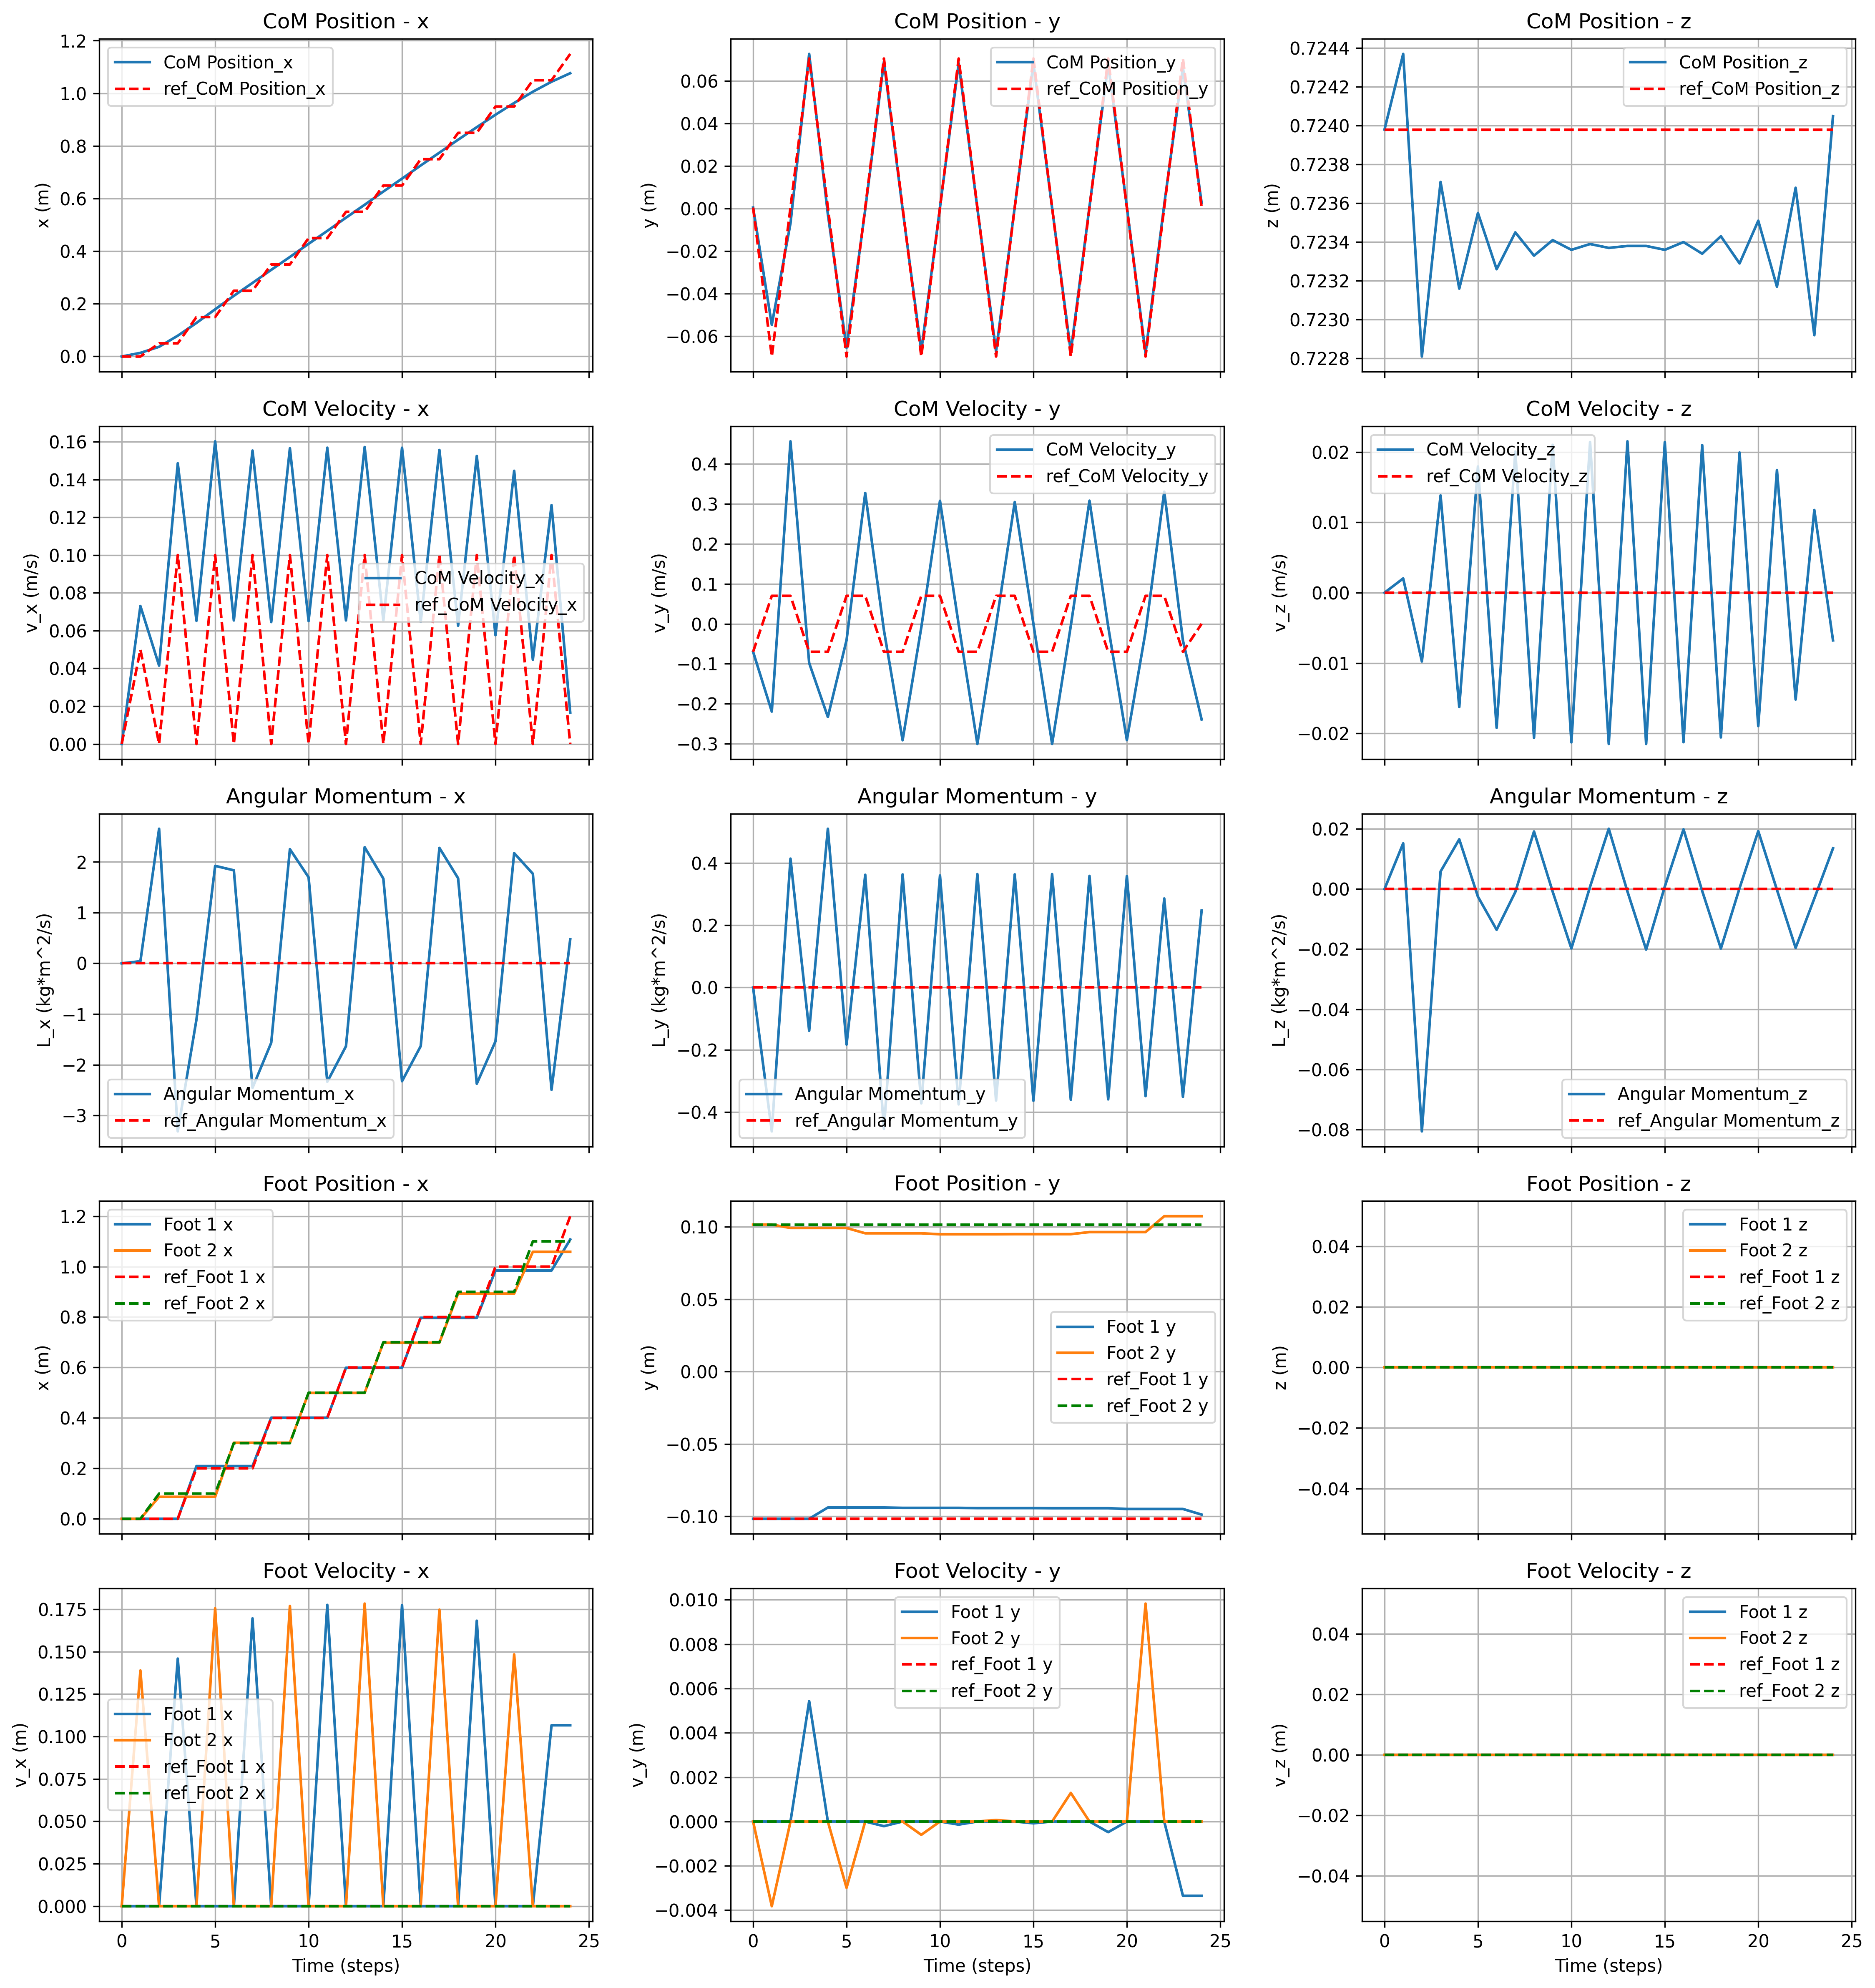
\includegraphics[width=0.8\textwidth]{C:/Users/giuse/OneDrive/Desktop/GITHUB PROJECTS/AMR-FP1/centroidal_dyn-main/plots/contact_x_walking.png}
    \caption{Trajectory vs Reference - Walking Task}
    \label{fig:yourlabel}
\end{figure}
\begin{table}[H]
    \centering
    \renewcommand{\arraystretch}{1.2}
    \resizebox{\textwidth}{!}{
        \begin{tabular}{c|c|c|c|c}
            \hline
            Interval & Right Foot (x,y,z) & Left Foot (x,y,z) & $\Sigma L_k$ & Sum Forces (x,y,z) \\
            \hline
            0 & (0.3186, 9.993, 49.064) & (0.3135, -8.822, 49.053) & (0, 0) & (0.6322, 1.1712, 98.1175) \\
            1 & (-2.9751, 12.258, 97.955) & (0, 0, 0) & (0, -1) & (-2.9751, 12.258, 97.9551) \\
            2 & (3.3303, -0.425, 48.897) & (-4.9023, -19.591, 49.650) & (0, 0) & (-1.5720, -20.016, 98.5473) \\
            3 & (0, 0, 0) & (-6.5058, 4.261, 97.490) & (-1, 0) & (-6.5058, 4.261, 97.4904) \\
            4 & (-7.0579, 14.053, 49.653) & (4.3045, -4.005, 49.156) & (0, 0) & (-2.7535, 10.048, 98.8092) \\
            5 & (-6.9692, 1.921, 97.308) & (0, 0, 0) & (0, -1) & (-6.9692, 1.921, 97.3081) \\
            6 & (3.0511, 1.817, 49.240) & (-5.6393, -16.023, 49.724) & (0, 0) & (-2.5882, -14.206, 98.9640) \\
            7 & (0, 0, 0) & (-6.7544, 0.511, 97.209) & (-1, 0) & (-6.7544, 0.511, 97.2091) \\
            8 & (-5.8989, 15.204, 49.739) & (3.3918, -2.610, 49.293) & (0, 0) & (-2.5070, 12.593, 99.0319) \\
            9 & (-6.8000, 0.593, 97.167) & (0, 0, 0) & (0, -1) & (-6.8000, 0.593, 97.1669) \\
            10 & (3.3444, 2.219, 49.301) & (-5.8685, -15.554, 49.761) & (0, 0) & (-2.5241, -13.335, 99.0619) \\
            11 & (0, 0, 0) & (-6.8143, -0.121, 97.149) & (-1, 0) & (-6.8143, -0.121, 97.1486) \\
            12 & (-5.9310, 15.393, 49.762) & (3.3932, -2.385, 49.310) & (0, 0) & (-2.5378, 13.008, 99.0720) \\
            13 & (-6.8282, 0.352, 97.144) & (0, 0, 0) & (0, -1) & (-6.8282, 0.352, 97.1443) \\
            14 & (3.3762, 2.297, 49.306) & (-5.9126, -15.492, 49.766) & (0, 0) & (-2.5364, -13.195, 99.0716) \\
            15 & (0, 0, 0) & (-6.8131, -0.182, 97.150) & (-1, 0) & (-6.8131, -0.182, 97.1495) \\
            16 & (-5.8724, 15.400, 49.756) & (3.3634, -2.397, 49.305) & (0, 0) & (-2.5091, 13.003, 99.0602) \\
            17 & (-6.7635, 0.425, 97.169) & (0, 0, 0) & (0, -1) & (-6.7635, 0.425, 97.1685) \\
            18 & (3.2848, 2.288, 49.282) & (-5.7111, -15.640, 49.747) & (0, 0) & (-2.4263, -13.351, 99.0282) \\
            19 & (0, 0, 0) & (-6.6265, 0.084, 97.216) & (-1, 0) & (-6.6265, 0.084, 97.2160) \\
            20 & (-5.4018, 15.280, 49.700) & (3.1738, -2.710, 49.254) & (0, 0) & (-2.2280, 12.571, 98.9543) \\
            21 & (-6.2994, 1.076, 97.326) & (0, 0, 0) & (0, -1) & (-6.2994, 1.076, 97.3264) \\
            22 & (2.6126, 2.308, 49.129) & (-4.3267, -16.682, 49.649) & (0, 0) & (-1.7142, -14.373, 98.7771) \\
            23 & (0, 0, 0) & (-5.5100, 1.696, 97.583) & (-1, 0) & (-5.5100, 1.696, 97.5828) \\
            \hline
        \end{tabular}
    }
    \caption{Summary of Forces and Foot Positions per Interval - Walking Task}
    \label{tab:data_table}
\end{table}
\begin{figure}[htbp]
    \centering
    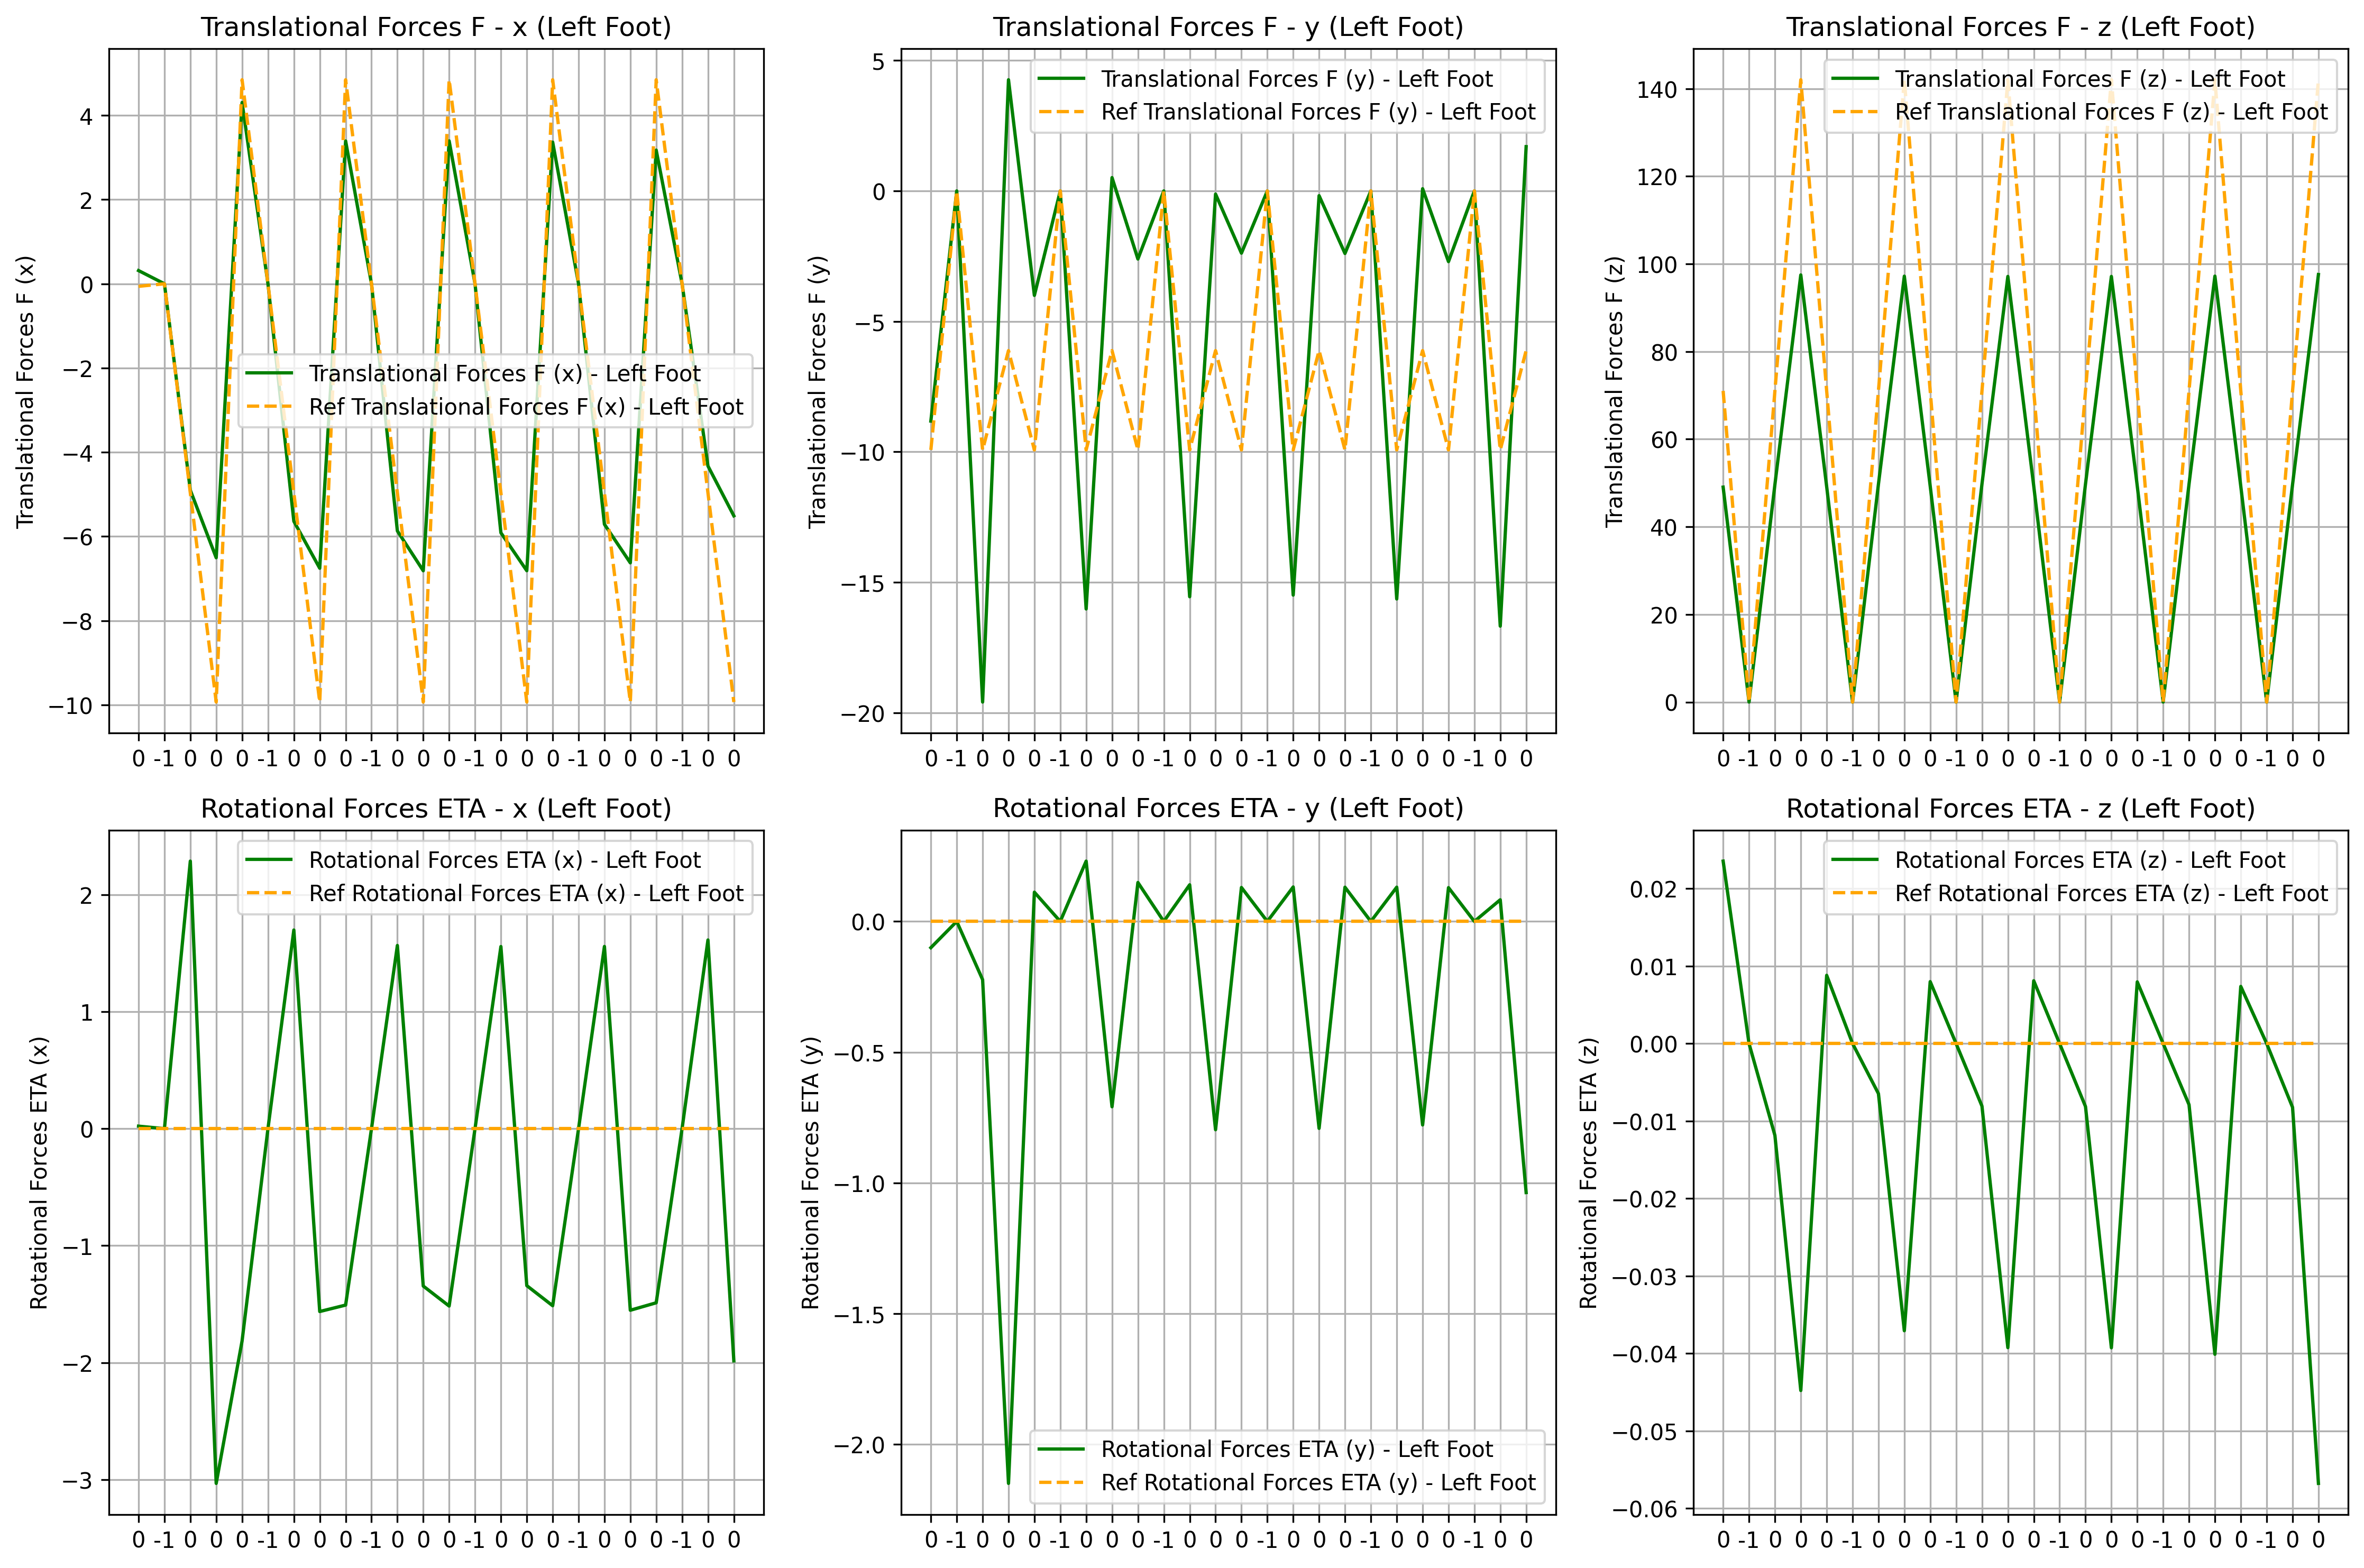
\includegraphics[width=0.8\textwidth]{C:/Users/giuse/OneDrive/Desktop/GITHUB PROJECTS/AMR-FP1/centroidal_dyn-main/plots/contact_forces_walking_right.png}
    \caption{Trajectory vs Reference Forces - Walking Task}
    \label{fig:contact_forces_walking_right}
\end{figure}
\begin{figure}[htbp]
    \centering
    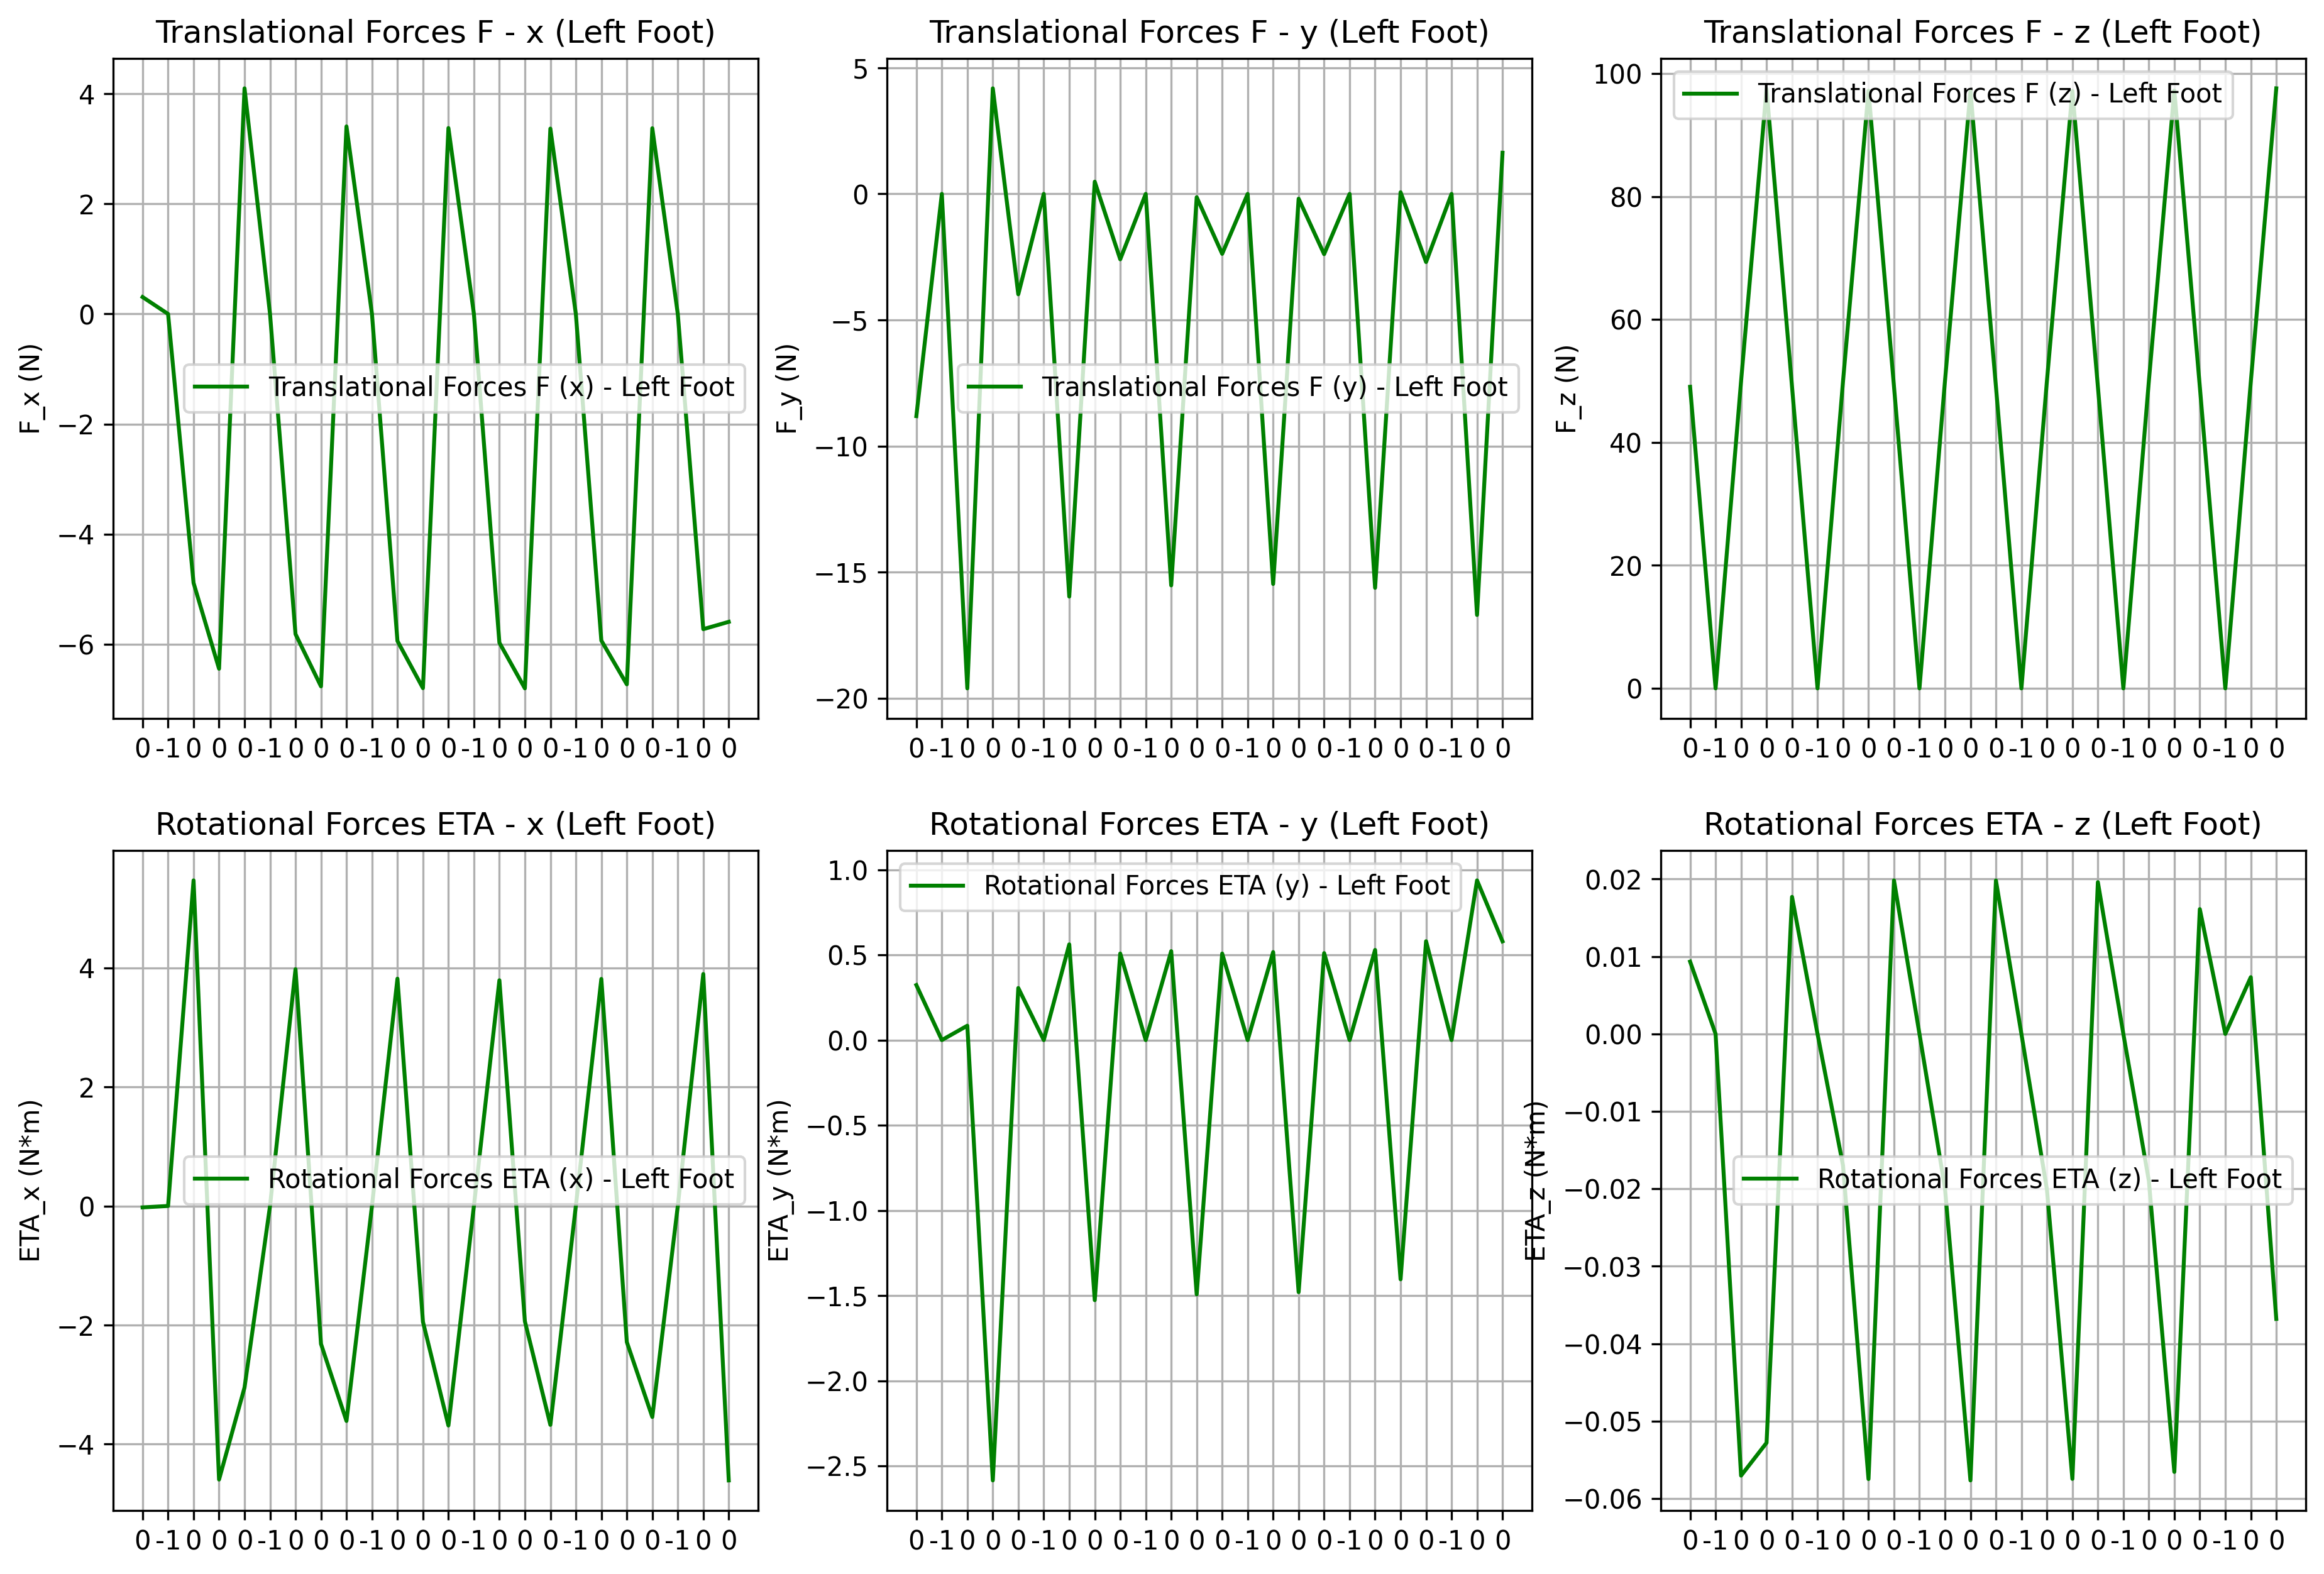
\includegraphics[width=0.8\textwidth]{C:/Users/giuse/OneDrive/Desktop/GITHUB PROJECTS/AMR-FP1/centroidal_dyn-main/plots/contact_forces_walking_left.png}
    \caption{Trajectory vs Reference Forces - Walking Task}
    \label{fig:contact_forces_walking_left}
\end{figure}


\paragraph{Simulation} 
Our work is built upon the repository available at [GitHub Link], which originally provides a comprehensive framework for simulating the HRP4 robot, including the dynamics model and control architecture. While the repository offers a complete baseline, we have extensively modified it by implementing our own dynamics and trajectory optimization framework. \\



\end{document}